%%
%% This is file `sample-sigconf-authordraft.tex',
%% generated with the docstrip utility.
%%
%% The original source files were:
%%
%% samples.dtx  (with options: `all,proceedings,bibtex,authordraft')
%% 
%% IMPORTANT NOTICE:
%% 
%% For the copyright see the source file.
%% 
%% Any modified versions of this file must be renamed
%% with new filenames distinct from sample-sigconf-authordraft.tex.
%% 
%% For distribution of the original source see the terms
%% for copying and modification in the file samples.dtx.
%% 
%% This generated file may be distributed as long as the
%% original source files, as listed above, are part of the
%% same distribution. (The sources need not necessarily be
%% in the same archive or directory.)
%%
%%
%% Commands for TeXCount
%TC:macro \cite [option:text,text]
%TC:macro \citep [option:text,text]
%TC:macro \citet [option:text,text]
%TC:envir table 0 1
%TC:envir table* 0 1
%TC:envir tabular [ignore] word
%TC:envir displaymath 0 word
%TC:envir math 0 word
%TC:envir comment 0 0
%%
%% The first command in your LaTeX source must be the \documentclass
%% command.
%%
%% For submission and review of your manuscript please change the
%% command to \documentclass[manuscript, screen, review]{acmart}.
%%
%% When submitting camera ready or to TAPS, please change the command
%% to \documentclass[sigconf]{acmart} or whichever template is required
%% for your publication.
%%
%% CAMBIAR AUTHORDRAFT A ACM
\documentclass[sigconf,ACM]{acmart}
%%
\usepackage{tikz}
\usetikzlibrary{positioning,arrows.meta,calc}

\usepackage{tabularx}
\usepackage{booktabs}
\usepackage{caption}
\usepackage{xcolor}
\usepackage{soul}
\sethlcolor{yellow}
\usepackage{array}
\usepackage{booktabs}
\graphicspath{{figs/}}
%% ELIMINAR COPYRIGHT PORTADA
\settopmatter{printacmref=false} % Elimina el bloque de citación de la izquierda
\setcopyright{none}              % Elimina el aviso de copyright
\renewcommand\footnotetextcopyrightpermission[1]{} % Limpia el pie de página
\pagestyle{plain}                % Asegura que no haya encabezados raros

%% \BibTeX command to typeset BibTeX logo in the docs
\AtBeginDocument{%
  \providecommand\BibTeX{{%
    Bib\TeX}}}

%% Rights management information.  This information is sent to you
%% when you complete the rights form.  These commands have SAMPLE
%% values in them; it is your responsibility as an author to replace
%% the commands and values with those provided to you when you
%% complete the rights form.
\setcopyright{acmlicensed}
\copyrightyear{2026}
\acmYear{2026}
\acmDOI{XXXXXXX.XXXXXXX}
%% These commands are for a PROCEEDINGS abstract or paper.
\acmConference[]{}{}{}
%% \acmConference[Conference acronym 'XX]{Make sure to enter the correct conference title from your rights confirmation email}{June 03--05, 2018}{Woodstock, NY}
%%
%%  Uncomment \acmBooktitle if the title of the proceedings is different
%%  from ``Proceedings of ...''!
%%
%%\acmBooktitle{Woodstock '18: ACM Symposium on Neural Gaze Detection,
%%  June 03--05, 2018, Woodstock, NY}
\acmISBN{978-1-4503-XXXX-X/2018/06}


%%
%% Submission ID.
%% Use this when submitting an article to a sponsored event. You'll
%% receive a unique submission ID from the organizers
%% of the event, and this ID should be used as the parameter to this command.
%%\acmSubmissionID{123-A56-BU3}

%%
%% For managing citations, it is recommended to use bibliography
%% files in BibTeX format.
%%
%% You can then either use BibTeX with the ACM-Reference-Format style,
%% or BibLaTeX with the acmnumeric or acmauthoryear sytles, that include
%% support for advanced citation of software artefact from the
%% biblatex-software package, also separately available on CTAN.
%%
%% Look at the sample-*-biblatex.tex files for templates showcasing
%% the biblatex styles.
%%

%%
%% The majority of ACM publications use numbered citations and
%% references.  The command \citestyle{authoryear} switches to the
%% "author year" style.
%%
%% If you are preparing content for an event
%% sponsored by ACM SIGGRAPH, you must use the "author year" style of
%% citations and references.
%% Uncommenting
%% the next command will enable that style.
%%\citestyle{acmauthoryear}


%%
%% end of the preamble, start of the body of the document source.
\begin{document}

%%
%% The "title" command has an optional parameter,
%% allowing the author to define a "short title" to be used in page headers.
\title{Redes Neuronales Guiadas por Física para la Estimación de Parámetros
Estelares desde Espectros H$\alpha$: Cerrando la Brecha del Dominio
Sintético-Observado en Estrellas Masivas}

%%
%% The "author" command and its associated commands are used to define
%% the authors and their affiliations.
%% Of note is the shared affiliation of the first two authors, and the
%% "authornote" and "authornotemark" commands
%% used to denote shared contribution to the research.
\author{Santiago Anwandter}
\affiliation{%
  \institution{Universidad Técnica Federico Santa María}
  \city{Valparaíso}
  \country{Chile}
}
\email{santiago.anwandter@usm.cl}

\author{Benjamín Cisternas}
\affiliation{%
  \institution{Universidad Técnica Federico Santa María}
  \city{Valparaíso}
  \country{Chile}}
\email{benjamin.cisternas@usm.cl}

%%
%% By default, the full list of authors will be used in the page
%% headers. Often, this list is too long, and will overlap
%% other information printed in the page headers. This command allows
%% the author to define a more concise list
%% of authors' names for this purpose.
\renewcommand{\shortauthors}{Anwandter et al.}

%%
%% The abstract is a short summary of the work to be presented in the
%% article.
\begin{abstract}
Estimar los parámetros estelares de estrellas masivas a partir de líneas espectrales H$\alpha$ es una tarea crítica para comprender la evolución estelar. Los modelos de aprendizaje automático entrenados en grandes grillas de espectros sintéticos logran un rendimiento sólido dentro de la distribución, pero se degradan severamente al aplicarse a espectros reales observados, un
fenómeno conocido como la \emph{brecha sintética}. Proponemos abordar esta limitación incorporando una restricción suave basada en física en la función de pérdida de entrenamiento, derivada de la prescripción autoconsistente de tasa de pérdida de masa de Figueroa-Tapia et al.~\cite{FigueroaTapia2026}. Nuestra hipótesis es que penalizar predicciones físicamente inconsistentes durante el entrenamiento reducirá los errores fuera de distribución en observaciones reales sin requerir datos pareados sintético-observados. Validamos esta hipótesis en tres niveles: el error in-distribution sobre una partición sintética de prueba, la coherencia distribucional contra espectros UVES~POP sin etiquetas, y el error puntual fuera de distribución contra las etiquetas parciales de literatura de estrellas de tipo O de los catálogos IACOB~\cite{Holgado2025,deBurgos2024}. El término físico reduce el error medio absoluto de $T_\mathrm{eff}$ sobre estrellas reales de ${\sim}10\,300$ a ${\sim}3\,500$\,K y revierte un sesgo sistemático de $+10\,000$\,K ---recolocando las predicciones dentro del régimen físico admisible---, confirmando la hipótesis sin emplear datos observados etiquetados durante el entrenamiento.
\end{abstract}

%%
%% The code below is generated by the tool at http://dl.acm.org/ccs.cfm.
%% Please copy and paste the code instead of the example below.
%%
\begin{CCSXML}
<ccs2012>
 <concept>
  <concept_id>10010147.10010257.10010293.10010294</concept_id>
  <concept_desc>Computing methodologies~Neural networks</concept_desc>
  <concept_significance>500</concept_significance>
 </concept>
</ccs2012>
\end{CCSXML}
\ccsdesc[500]{Computing methodologies~Neural networks}

%%
%% Keywords. The author(s) should pick words that accurately describe
%% the work being presented. Separate the keywords with commas.
\keywords{physics-guided machine learning, massive stars, H$\alpha$, synthetic gap, domain adaptation}
%% A "teaser" image appears between the author and affiliation
%% information and the body of the document, and typically spans the
%% page.
\begin{teaserfigure}
  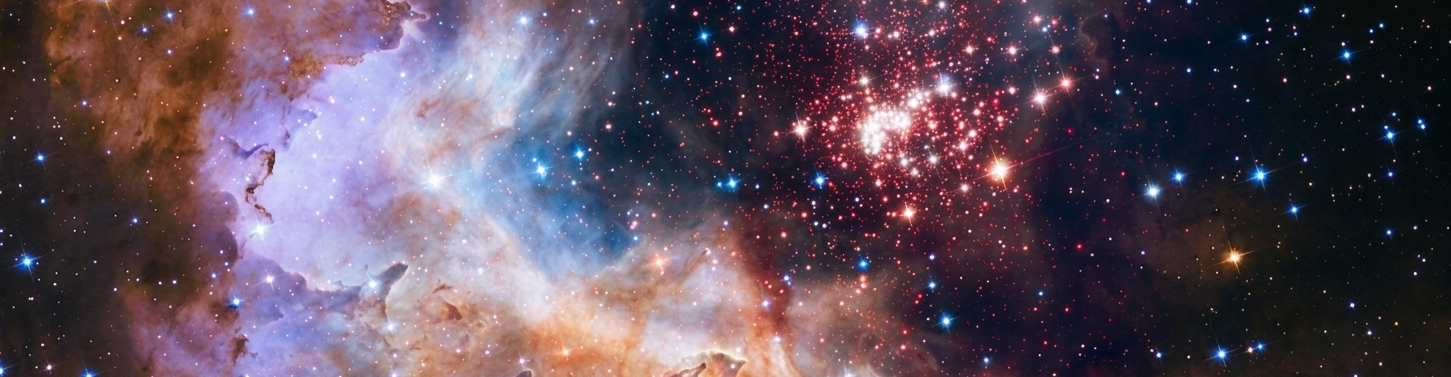
\includegraphics[width=\textwidth]{teaser.png}
  \label{fig:teaser}
\end{teaserfigure}

%%
%% This command processes the author and affiliation and title
%% information and builds the first part of the formatted document.
\maketitle

\section{Introducción}
Las estrellas masivas gobiernan la evolución química de las galaxias a través de poderosos vientos impulsados por radiación y supernovas de colapso de núcleo. Caracterizar sus parámetros de tasa de pérdida de masa $\dot{M}$ y parámetros atmosféricos como temperatura efectiva $T_\mathrm{eff}$, gravedad superficial $\log g$ es esencial para modelos evolutivos precisos \cite{FigueroaTapia2026}. La línea H$\alpha$ es el diagnóstico espectroscópico principal para los parámetros de viento en supergigantes de tipo O, ya que la forma de su perfil es directamente sensible tanto a la velocidad terminal del viento $v_\infty$ como a la propia tasa de pérdida de masa $\dot{M}$~\cite{Ortiz2025}.

Trabajos recientes han demostrado que el aprendizaje automático puede estimar los parámetros estelares a partir de perfiles H$\alpha$. Ortiz et al.~\cite{Ortiz2025} desarrollaron un pipeline de múltiples etapas que combina agrupamiento por Gaussian Mixture Models, clasificación por redes neuronales
profundas y deconvolución espectral entrenado en la base de datos sintética ISOSCELES~\cite{Ortiz2025}, logrando inferencia en menos de un segundo y superando el ajuste de expertos para 9 de las 12 supergigantes de tipo B evaluadas. Sin embargo, un desafío fundamental permanece sin resolver: los modelos entrenados completamente en espectros sintéticos típicamente fallan al generalizarse a observaciones reales. Esta es la \emph{brecha sintética}, una discrepancia sistemática entre perfiles de líneas teóricos y observados que surge de las suposiciones simplificadoras en los modelos de atmósfera, efectos instrumentales y ruido observacional~\cite{OBriain2021}. La Figura~\ref{fig:synthgap} ilustra esta discrepancia a nivel de perfil espectral: el perfil sintético es sistemáticamente más profundo y suave que su contraparte observada.

\begin{figure}[t]
  \centering
  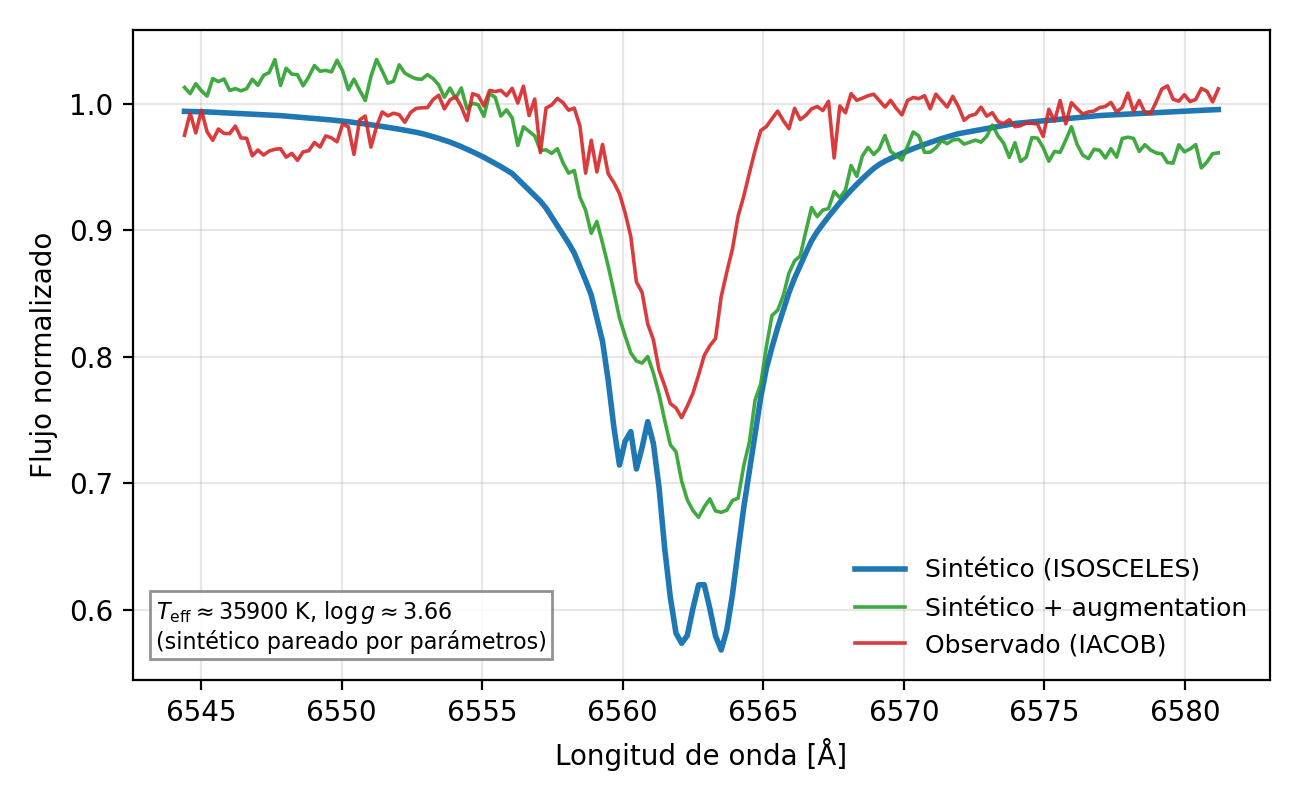
\includegraphics[width=\columnwidth]{fig_synthetic_gap.png}
  \caption{Brecha sintético--observado en H$\alpha$. Perfil sintético ISOSCELES
  (azul) frente a su contraparte observada de IACOB (rojo, HD\,41997), ambos con
  parámetros próximos ($T_\mathrm{eff}\approx 35\,900$\,K, $\log g\approx 3.66$).
  El núcleo sintético es más profundo y carece del ensanchamiento, \emph{veiling},
  asimetría y ruido ---incluidas líneas metálicas--- presentes en la observación.
  La augmentación (verde) cierra parte de la brecha pero no su totalidad,
  motivando la restricción física.}
  \label{fig:synthgap}
\end{figure}

La consecuencia es que un regresor entrenado en la grilla ISOSCELES produce estimaciones de parámetros físicamente implausibles al evaluarse en espectros estelares observados. Las predicciones caen fuera de la región físicamente admisible del espacio de parámetros, haciendo al modelo poco confiable para datos reales. Esto motiva la pregunta central de este trabajo.

\textbf{Pregunta de Investigación.} 
¿Puede un modelo de machine learning entrenado exclusivamente con espectros de $H_\alpha$ sintéticos generalizar de forma físicamente consistente a espectros observados de estrellas masivas de tipo O, si se incorpora una restricción física teórica autoconsistente en la función de pérdida? Precisamos el sentido operacional de \emph{físicamente consistente}: medimos dos propiedades verificables ---que las predicciones caigan dentro del rango admisible del régimen O y que se corrija el sesgo sistemático respecto a las etiquetas de literatura--- sin afirmar por ello una mejora en la exactitud por estrella individual.

\textbf{Hipótesis.} Una red neuronal entrenada en perfiles H$\alpha$ sintéticos con un término de pérdida física auxiliar que penaliza desviaciones de la prescripción autoconsistente de pérdida de masa de Figueroa-Tapia et al.~\cite{FigueroaTapia2026} producirá predicciones de parámetros estelares que sean más consistentes físicamente y generalicen mejor a espectros observados \emph{de estrellas masivas de tipo O} que una línea de base puramente basada en datos entrenada con los mismos datos sintéticos, incluso sin acceso a etiquetas observadas durante el entrenamiento.

Esta hipótesis es directamente comprobable: la restricción física es una ecuación algebraica que relaciona tres de las cuatro salidas predichas por nuestro modelo $\{T_\mathrm{eff}, \log g, R_*\}$ con la cuarta, $\dot{M}$ (ver §\ref{subsec:formalizacion}), y puede evaluarse tanto en entradas sintéticas como observadas sin ningún dato adicional etiquetado. Adicionalmente, disponemos de etiquetas de literatura parciales del proyecto IACOB: Holgado et al.~\cite{Holgado2025} proporcionan $T_{\mathrm{eff}}$, $\log g$ y $R_*$ para 358 estrellas de tipo O, mientras que de~Burgos et al.~\cite{deBurgos2024} proporcionan $T_{\mathrm{eff}}$ y $\log g$ para 527 estrellas O y B tempranas; tras aplicar el filtro de validez FT26 (§\ref{subsec:datos}) conservamos únicamente el subconjunto O. Esto permite una evaluación OOD con métricas de error directo (MAE, RMSE, sesgo).
\subsection*{Relevancia e Impacto}

\paragraph{Impacto científico.} La brecha sintética en espectroscopía estelar limita la explotación de grandes surveys fotométricos y espectroscópicos (GAIA, SDSS, VLT-FLAMES) para estudios de población de estrellas masivas. Si una restricción física autoconsistente permite reducir el error de dominio sin requerir datos pareados sintético-observados, se elimina un cuello de botella fundamental en la caracterización de vientos estelares. Por ejemplo, censos de estrellas O como el VLT-FLAMES Tarantula Survey o el propio proyecto IACOB ---hoy dependientes de ajuste manual estrella a estrella--- podrían procesarse de forma homogénea y rápida, habilitando estudios poblacionales de la relación viento--metalicidad. Esto impacta directamente modelos de evolución estelar, síntesis de poblaciones y retroalimentación química en simulaciones cosmológicas.

\paragraph{Impacto social y tecnológico.} Las estrellas masivas son los principales productores de elementos pesados y radiación ionizante; comprender sus parámetros de viento es esencial para modelar la habitabilidad planetaria y la evolución galáctica. Desde una perspectiva de machine learning, este trabajo ofrece un caso de estudio sobre cómo integrar conocimiento científico de primer principio en redes neuronales profundas cuando los datos etiquetados del dominio objetivo son inexistentes, una situación común en astrofísica, geofísica e ingeniería.

\paragraph{Beneficiarios.} La comunidad de astrofísica estelar obtiene una herramienta de inferencia rápida y físicamente consistente; la comunidad de ML recibe una demostración de \emph{physics-guided deep learning} en un régimen de cambio de dominio severo donde las técnicas estándar de adaptación de dominio no aplican por ausencia de datos observacionales etiquetados.

\paragraph{Reproducibilidad.} Código, resultados y modelos entrenados disponibles en \url{https://github.com/sanwandter/pgnn-stellar-parameter}.

\section{Related Work}

\subsection{Neural Networks para la Estimación de Parámetros Estelares desde H$\alpha$}

Ortiz et al.~\cite{Ortiz2025} es el predecesor más directo de este trabajo y emplea la misma infraestructura de datos. Su método de múltiples etapas utiliza perfiles H$\alpha$ sintéticos de la grilla ISOSCELES de soluciones de viento m-CAK $\delta$-slow para entrenar un clasificador de red neuronal profunda que asigna un perfil espectral observado a uno de 21 grupos. Una comparación $\chi^2$ posterior dentro del grupo predicho identifica el modelo de mejor ajuste. El método es objetivo, rápido y mejora el ajuste manual para la mayoría de su muestra de supergigantes B.

Ortiz et al. sí evalúan el método en espectros observados, pero \emph{sin adaptación explícita al cambio de dominio}: la evaluación se realiza en estrellas con parámetros estelares \emph{conocidos a priori} de estudios anteriores, proporcionando una cota superior de factibilidad. La pregunta de qué sucede cuando el modelo se aplica sin conocimiento previo, en el régimen fuera de distribución, no se aborda. Los autores reconocen que 3 de las 12 estrellas arrojaron ajustes insatisfactorios, y que el método no estima incertidumbres de parámetros desde un punto de vista estadístico, reservando las redes neuronales bayesianas para trabajo futuro.

Nuestro trabajo extiende esta línea de investigación apuntando explícitamente al fallo de generalización: en lugar de aceptar la brecha sintética como una limitación, proponemos reducirla mediante entrenamiento informado por física.

\subsection{La Brecha Sintética en Espectroscopía Estelar}

O'Briain et al.~\cite{OBriain2021} proporcionan la caracterización más rigurosa de la brecha sintética en el contexto de la espectroscopía estelar. Su método Cycle-StarNet aplica adaptación de dominio no supervisada basada en redes generativas antagónicas y representaciones latentes compartidas para transferir modelos sintéticos de Kurucz al dominio observacional de APOGEE (Apache Point Observatory Galactic Evolution Experiment). Demuestran que incluso con una lista de líneas mejorada, los modelos Kurucz crudos producen un residuo normalizado considerable contra las observaciones de APOGEE, que Cycle-StarNet logra reducir drásticamente, alcanzando una mejora sustancial en el $\chi^2_R$ reducido.

Es importante destacar que el enfoque de adaptación de dominio de Cycle-StarNet es completamente basado en datos: requiere grandes conjuntos de datos observados no etiquetados y no codifica explícitamente física de vientos estelares o atmósfera. Esto es a la vez una fortaleza (no se necesita conocimiento del dominio) y una limitación: no hay garantía de que las predicciones adaptadas al dominio caigan dentro del espacio de parámetros físicamente admisible, particularmente para tipos estelares fuera de distribución. Además, Cycle-StarNet fue diseñado para la estimación de abundancias en estrellas de tipo solar; su aplicabilidad a estrellas masivas con perfiles H$\alpha$ complejos formados por vientos no ha sido demostrada.

La comprensión central de~\cite{OBriain2021} para nuestro trabajo es el diagnóstico preciso del problema: la brecha sintética en H$\alpha$ para estrellas masivas probablemente está impulsada por la misma combinación de aproximaciones del modelo y efectos instrumentales identificados para estrellas más frías, y debe abordarse en lugar de asumirse inexistente.

\subsection{Physics informed neural networks}

Von Rueden et al.~\cite{vonRueden2021} proporcionan el marco conceptual para nuestra solución propuesta a través de una taxonomía exhaustiva del aprendizaje automático informado. Definen el \emph{Informed machine learning} como el aprendizaje a partir de una fuente de información híbrida de datos y conocimiento previo, donde el conocimiento previo se integra explícitamente en el pipeline de aprendizaje. Entre las estrategias de integración identificadas, incorporar física en forma de \emph{ecuaciones algebraicas en el algoritmo de aprendizaje mediante términos de pérdida basados en conocimiento} representa el enfoque dominante para el conocimiento científico. Esta estrategia de agregar un término de penalización $\lambda_k \mathcal{L}_k(f(\mathbf{x}_i), \mathbf{x}_i)$ a la pérdida estándar se ha aplicado en dominios que van desde la dinámica de fluidos hasta la predicción de temperatura del agua, donde consistentemente mejora la generalización y asegura la consistencia con las leyes físicas conocidas.

Masclans et al.~\cite{Masclans2023} proporcionan una prueba de concepto directa en un problema de regresión termofísica análogo. Su Red Neuronal Informada por Termodinámica (TINN) reconstruye campos de temperatura y densidad a partir de datos de velocidad de flujos turbulentos supercríticos mediante la incorporación de la ecuación de estado de gas real como término de penalización suave en la función de pérdida. Su resultado clave es que en el escenario de generalización difícil (Caso II: datos de entrenamiento y prueba de instantáneas temporalmente distantes con diferentes perfiles termofísicos), la línea de base ANN puramente basada en datos se degrada significativamente, mientras que TINN recupera los perfiles correctos para la región de pared caliente. La restricción física proporciona la regularización necesaria para permanecer en la variedad físicamente admisible cuando la distribución de entrada cambia, exactamente el papel que buscamos para el cambio de dominio sintético-real en espectroscopía
H$\alpha$.

Tanto~\cite{vonRueden2021} como~\cite{Masclans2023} establecen que los términos de pérdida informados por física son más efectivos precisamente en el régimen de datos limitados o cambio distribucional, que caracteriza nuestro problema.

\subsection{PINNs en Astrofísica Estelar}
\label{subsec:pinns-astro}

Ballester et al.~\cite{Ballester2026} presentan la primera demostración de un marco PINN auto-supervisado para las ecuaciones de estructura estelar, combinando pérdidas basadas en las ecuaciones diferenciales de equilibrio hidrostático y térmico con redes auxiliares diferenciables para la ecuación de estado y la opacidad. El modelo produce perfiles radiales continuos de presión, temperatura, densidad y luminosidad sin requerir datos de entrenamiento etiquetados, alcanzando un error relativo medio de $3.06\%$ y $R^2 = 0.9998$ frente a soluciones de referencia del código MESA.

El resultado clave de~\cite{Ballester2026} para nuestro trabajo es su estudio de ablación sobre el papel de la restricción física. Los autores comparan tres configuraciones con la misma arquitectura: (a) entrenamiento puramente supervisado en datos MESA sin pérdida física, logrando $\mathrm{MRAE} = 3.85\%$; (b) entrenamiento supervisado con pérdida física incorporada, logrando $2.05\%$; y (c) entrenamiento auto-supervisado sin datos, usando únicamente la pérdida física, logrando $3.06\%$. La incorporación de la restricción física reduce el error en un $47\%$ respecto al modelo puramente basado en datos, y elimina oscilaciones no físicas en las predicciones. Los autores concluyen explícitamente que los enfoques de ML supervisado para modelado estelar ``heredan sesgos de las simulaciones subyacentes y no generalizan de forma fiable más allá de su dominio de entrenamiento''~\cite{Ballester2026}, diagnóstico que es análogo al problema de la brecha sintética que motiva nuestro trabajo.

Nuestro enfoque difiere del de~\cite{Ballester2026} en tres dimensiones. Primero, Ballester et al. abordan el \emph{problema directo}: dadas las condiciones de frontera, resolver la estructura interna de la estrella; nosotros abordamos el \emph{problema inverso}: dado un espectro observado, inferir los parámetros superficiales. Segundo, su restricción física consiste en residuos de PDEs evaluados mediante autodiferenciación; la nuestra es una relación algebraica cerrada derivada de la prescripción de pérdida de masa CNO, que no requiere derivadas de la red respecto a las entradas. Tercero, su marco es completamente auto-supervisado (sin etiquetas); el nuestro combina supervisión sobre la grilla sintética con una restricción física que actúa como regularizador de dominio. Esta distinción es deliberada: disponemos de etiquetas sintéticas de alta calidad y el objetivo no es reemplazar el solver, sino reducir la degradación al pasar de espectros sintéticos a observados.

\subsection{Prescripciones Autoconsistentes de Pérdida de Masa para Estrellas
Masivas}

Figueroa-Tapia et al.~\cite{FigueroaTapia2026} derivan prescripciones teóricas de tasa de pérdida de masa para estrellas de tipo O a través de una metodología autoconsistente que acopla la hidrodinámica del viento m-CAK con cálculos detallados de aceleración de líneas de radiación. Su hallazgo clave es que la prescripción de Vink et al. \cite{vink2000new} de uso común sobreestima las tasas de pérdida de masa porque subestima la dilución del flujo UV causada por líneas metálicas. Su prescripción de grilla-CNO, ajustada mediante regresión lineal bayesiana con $R^2 = 0.929$, relaciona $\dot{M}$ directamente con los parámetros estelares observables:
\begin{equation}
\begin{split}
  \log \dot{M}_\mathrm{FT26} = &\,(-20.74 \pm 0.61) + (1.44 \pm 0.09)\,\log\!\left(\frac{R_*}{R_\odot}\right) \\
  &- (3.85 \pm 0.15)\,\log g + (16.81 \pm 0.45)\,\log\!\left(\frac{T_\mathrm{eff}}{1000\,\mathrm{K}}\right),
\end{split}
\label{eq:cno_uncert}
\end{equation}
con $R^2 = 0.929$ sobre la muestra de ajuste de Figueroa-Tapia et al.~\cite{FigueroaTapia2026}.

Esta relación algebraica es precisamente el tipo de conocimiento científico identificado por~\cite{vonRueden2021} como más naturalmente representado e integrado como una restricción en la función de pérdida. Dado que la relación involucra solo cantidades predichas por nuestro modelo ($T_\mathrm{eff}$,
$\log g$, $R_*$, $\dot{M}$), no se necesitan entradas adicionales. La restricción es diferenciable con respecto a todas las salidas predichas y puede retropropagarse directamente.

\subsection{Brecha de Investigación}

Hasta donde sabemos, ningún trabajo previo ha combinado restricciones físicas de la teoría de vientos estelares con el entrenamiento de redes neuronales para reducir la brecha sintético-observado específicamente para la estimación de parámetros H$\alpha$ en estrellas masivas. Ortiz et al.~\cite{Ortiz2025} operan completamente dentro del dominio sintético; O'Briain et al.~\cite{OBriain2021} usan adaptación de dominio sin física; Masclans et al.~\cite{Masclans2023} y Ballester et al.~\cite{Ballester2026} usan restricciones físicas en dominios distintos al nuestro, termodinámica de fluidos y estructura estelar interna, respectivamente, y ninguno aborda el problema inverso de estimación de parámetros superficiales desde espectros H$\alpha$ bajo cambio de dominio sintético-real.

\section{Metodología}
\label{sec:metodologia}

\subsection{Notación y formulación del problema}
\label{subsec:formalizacion}

Sea un espectro estelar en la región H$\alpha$ ---definida como la ventana $[6542.8, 6582.8]$\,Å (${\pm}20$\,Å en torno a la línea H$\alpha$, $6562.8$\,Å)--- muestreado en $N=200$ puntos equiespaciados ($\Delta\lambda\approx0.2$\,Å/px), representado como un vector de flujo normalizado $\mathbf{x} \in \mathbb{R}^{N}$. Los espectros observados provienen de instrumentos de alta resolución ($R\gtrsim40\,000$; FIES, FEROS, HERMES, UVES) y se degradan a esta grilla común mediante el re-muestreo. El objetivo es predecir un vector de parámetros estelares $\mathbf{y} = [T_{\mathrm{eff}}, \log g, \log \dot{M}, R_{*}]^{\top} \in \mathbb{R}^{4}$, donde $T_{\mathrm{eff}}$ es la temperatura efectiva, $\log g$ la gravedad superficial, $\log \dot{M}$ el logaritmo de la tasa de pérdida de masa, y $R_{*}$ el radio estelar.

Denotamos el conjunto de entrenamiento sintético como $\mathcal{D}_{\mathrm{syn}} = \{(\mathbf{x}_i, \mathbf{y}_i)\}_{i=1}^{N_{\mathrm{syn}}}$, donde las etiquetas $\mathbf{y}_i$ provienen de la grilla ISOSCELES de modelos de viento m-CAK $\delta$-slow. El conjunto de evaluación observacional, sin etiquetas de entrenamiento, es $\mathcal{D}_{\mathrm{obs}} = \{\mathbf{x}_j\}_{j=1}^{N_{\mathrm{obs}}}$, correspondiente a espectros de la encuesta ESO UVES~POP.

Dado que los rangos de los parámetros difieren en órdenes de magnitud, aplicamos una normalización Min-Max a cada componente:
\begin{equation}
  \tilde{y}_k = \frac{y_k - y_k^{\min}}{y_k^{\max} - y_k^{\min}}, \quad k \in \{T_{\mathrm{eff}}, \log g, \log \dot{M}, R_{*}\},
  \label{eq:minmax}
\end{equation}
donde $y_k^{\min}$ y $y_k^{\max}$ se computan exclusivamente sobre $\mathcal{D}_{\mathrm{syn}}$: $T_{\mathrm{eff}}\in[30\,000,45\,000]$\,K, $\log g\in[3.15,3.90]$, $\log\dot{M}\in[-10.47,-5.25]$ y $R_*\in[7.02,20.93]\,R_\odot$. Estos mismos rangos se emplean para desnormalizar las predicciones antes de evaluar $\mathcal{L}_{\mathrm{phys}}$ en espacio físico (§\ref{subsec:loss}).

\subsection{Datos y preprocesamiento}
\label{subsec:datos}

\begin{table}[ht]
  \caption{Conjuntos de datos efectivamente utilizados. $N$: número de
    espectros. ISOSCELES es el subconjunto de tipo O no-rotante válido bajo los
    rangos FT26 de la grilla completa ($342\,779$). IACOB fusiona los catálogos
    de Holgado2025 y de~Burgos2024 tras el filtro de validez FT26
    ($184/522$ estrellas; $148$ con $R_*$).}
  \label{tab:datasets}
  \small
  \setlength{\tabcolsep}{3pt}
  \begin{tabular}{@{}l l >{\raggedright\arraybackslash}p{2.3cm} >{\raggedright\arraybackslash}p{2.0cm}@{}}
    \toprule
    \textbf{Conjunto} & \textbf{$N$} & \textbf{Etiquetas} & \textbf{Uso} \\
    \midrule
    ISOSCELES (sint.) & 33\,444 & $T_{\mathrm{eff}}, \log g, \log \dot{M}, R_{*}$ & Entren./Valid./Test \\
    UVES~POP O (obs.) & 12 & Ninguna & Eval. OOD distribucional ($W_1$) \\
    IACOB (filtro FT26) & 184 & $T_{\mathrm{eff}}, \log g$; $R_*$ (148) & Eval. OOD puntual \\
    \bottomrule
  \end{tabular}
\end{table}

\paragraph{Espectros sintéticos (ISOSCELES)}
La grilla ISOSCELES~\cite{Ortiz2025} contiene $342\,779$ espectros H$\alpha$ sintéticos generados mediante el código de transferencia radiativa FASTWIND acoplado con soluciones hidrodinámicas m-CAK $\delta$-slow, cubriendo rangos de temperatura efectiva $T_{\mathrm{eff}}$, gravedad superficial $\log g$, tasa de pérdida de masa $\log \dot{M}$ y radio estelar $R_*$. De esta grilla seleccionamos el subconjunto de $33\,444$ espectros de tipo O no-rotantes cuyos parámetros caen dentro de los rangos de validez de la prescripción FT26, sobre el que se realiza la partición de entrenamiento, validación y prueba.%

\paragraph{Espectros observacionales sin etiquetas (ESO UVES~POP)}
Utilizamos espectros de estrellas masivas de la biblioteca espectral
ESO UVES Paranal Observatory Project, observados con el
espectrógrafo UVES del VLT. Se seleccionan
estrellas con tipos espectrales O. El preprocesamiento es
idéntico al sintético: recorte a la región H$\alpha$, re-muestreo a
$N = 200$ puntos mediante interpolación lineal, y normalización.
Este conjunto se utiliza exclusivamente para evaluación distributiva OOD, sin
etiquetas de parámetros estelares.

\paragraph{Espectros observacionales con etiquetas (IACOB)}
El proyecto IACOB provee dos catálogos complementarios de parámetros
espectroscópicos:

Holgado et al.~\cite{Holgado2025} analizan 358 estrellas galácticas de
tipo O combinando espectroscopía de alta resolución con paralajes Gaia DR3 y
fotometría multibanda. Reportan $T_{\mathrm{eff}}$, gravedad superficial $\log g$, radio estelar $R_*$, entre otros. Los instrumentos principales son FIES (Nordic Optical Telescope), FEROS (MPG/ESO 2.2m) y HERMES.

De~Burgos et al.~\cite{deBurgos2024} analizan 527 estrellas OB luminosas
galácticas con FASTWIND, reportando $T_{\mathrm{eff}}$, $\log g$, y el parámetro de fuerza de viento $\log Q = \log[\dot{M}/(v_\infty R_*)^{3/2}]$.

\paragraph{Filtro de validez FT26.}
Para que la evaluación puntual se realice dentro del régimen de validez de la
prescripción CNO, restringimos la muestra IACOB combinada a estrellas con
$T_\mathrm{eff} \in [30\,000, 50\,000]$\,K, $\log g \in [2.9, 4.3]$ y, cuando
$R_*$ está disponible, $R_* \in [7, 70]\,R_\odot$. De las $522$ estrellas con
espectro H$\alpha$ válido, $184$ superan el filtro y constituyen el conjunto de
evaluación puntual; $148$ de ellas disponen de $R_*$. Estos rangos coinciden con
los empleados para definir la tasa de predicciones fuera de rango físico
(§\ref{subsec:protocolo}).

Todos los espectros IACOB se preprocesan siguiendo el mismo pipeline que los
datos sintéticos: recorte a la región H$\alpha$, re-muestreo a $N = 200$
puntos, y normalización. Este conjunto se mantiene completamente separado del entrenamiento. El cruce espectro--parámetros se realiza por identificador de estrella, y tanto la fusión de catálogos como el filtro FT26 se fijan \emph{a priori}, antes de cualquier evaluación del modelo. De las $184$ estrellas O válidas, $116$ provienen sólo de Holgado et al.~\cite{Holgado2025}, $36$ sólo de de~Burgos et al.~\cite{deBurgos2024} y $32$ son comunes a ambos catálogos; estas últimas se fusionan en una única entrada (sin duplicados), y los desacuerdos sistemáticos entre ambos \emph{pipelines} se asumen como un piso de ruido en las etiquetas (§\ref{sec:discusion}).

\paragraph{Aumento de datos.}
Dado el tamaño limitado de la grilla sintética, aplicamos data augmentation
físicamente motivada para simular efectos instrumentales y atmosféricos:
desplazamiento Doppler aleatorio ($\pm 5$\,px), ensanchamiento gaussiano
($\sigma \in [0, 2.5]$\,px), \emph{veiling} continuo
($f_v \in [0, 0.2]$), deformación polinomial del continuo, offset vertical ($\leq 0.01$), y ruido aditivo compuesto por una componente correlacionada de baja frecuencia más ruido blanco suavizado.
Cada espectro se replica 4 veces con augmentaciones independientes, resultando
en un conjunto de entrenamiento efectivo de ${\sim}4 \times 0.8 \times
N_{\mathrm{syn}}$ muestras.

\paragraph{Mismatch rotacional sintético-observado.}
La grilla ISOSCELES contiene perfiles H$\alpha$ sintéticos generados \emph{sin rotación estelar}, mientras que las observaciones de estrellas masivas presentan ensanchamiento rotacional con $v\sin i$ típicamente entre 50 y 300\,km/s para estrellas O~\cite{Holgado2025} y de Burgos~\cite{deBurgos2024}. Este mismatch es una fuente conocida de degradación: Ortiz et al.~\cite{Ortiz2025} lo manejan deconvolucionando los espectros observados antes de la clasificación. En nuestro pipeline adoptamos la estrategia opuesta: en lugar de deconvolucionar observaciones, incluimos en la augmentación sintética un ensanchamiento gaussiano con $\sigma \in [0, 2.5]$\,px que actúa como un proxy del ensanchamiento rotacional sumado a efectos instrumentales. Reconocemos que el kernel gaussiano no captura la forma exacta del perfil de rotación, por lo que esta es una aproximación de primer orden. Una mejora natural, que dejamos como trabajo futuro, es convolucionar con kernels rotacionales realistas usando $v\sin i$ muestreado de la distribución empírica de los catálogos IACOB.

\subsection{Arquitectura de red neuronal}
\label{subsec:arquitectura}

Empleamos una red neuronal convolucional residual 1D (ResNet-1D) como encoder espectral, motivada por los resultados de Cvrček et al.~\cite{Cvrcek2025} quienes demostraron que arquitecturas ResNet superan consistentemente a CNNs puras en la reconstrucción de líneas de absorción en espectros de alta resolución (HARPS). En particular, Cvrček et al. reportan que deencoderes ResNet alcanzan errores de reconstrucción $0.0064 \pm 0.0011$ frente a $0.0139 \pm 0.0026$ de CNNs estándar, atribuyendo esta ventaja a las conexiones residuales que mitigan la dilución de información en capas profundas~\cite[Sect.~4.2.1]{Cvrcek2025}. Una ablación arquitectónica directa sobre nuestro problema ---un MLP o una CNN sin conexiones residuales como líneas de base--- queda como trabajo futuro; aquí nos apoyamos en esta evidencia externa para justificar la elección de ResNet-1D.

La arquitectura consta de los siguientes componentes:

\paragraph{Codificador ResNet-1D} La entrada $\mathbf{x} \in \mathbb{R}^{200 \times 1}$ (espectro unicanal) se procesa mediante:
\begin{enumerate}
  \item Una convolución inicial $\mathrm{Conv1D}(32, 7, \text{stride}=2)$ seguida de BatchNorm y ReLU.
  \item Tres bloques residuales 1D con progresión de canales $(32 \to 64 \to 128)$; los dos últimos cambian la dimensión de canales y emplean un atajo de proyección $1\times1$. Todos los bloques preservan la longitud espacial ($\text{stride}=1$); la reducción espacial proviene de la convolución inicial ($\text{stride}=2$) y del \emph{Global Average Pooling}.
  \item \emph{Global Average Pooling} 1D para reducir a un vector de características.
  \item Capa densa de \emph{bottleneck} con $\mathrm{latent\_dim}=64$ y activación ReLU.
\end{enumerate}

Cada bloque residual implementa la identidad clásica de He et al.~\cite{He2016} adaptada a convoluciones unidimensionales:
\begin{equation}
  \mathbf{h}_{l+1} = \sigma\left( \mathcal{F}(\mathbf{h}_l; \{W_l\}) + \mathbf{h}_l \right),
  \label{eq:residual}
\end{equation}
donde $\mathcal{F}$ representa dos convoluciones 1D de tamaño (\emph{kernel}) $3$ con BatchNorm intermedio, y $\sigma$ es ReLU. Cuando las dimensiones espaciales o de canales difieren, la conexión \emph{shortcut} se proyecta mediante convolución $1\times1$ con stride apropiado. La Figura~\ref{fig:modelo-full} resume el encoder, las cuatro cabezas multitarea y el flujo de ambos términos de pérdida.

\begin{figure*}[t]
  \centering
  \resizebox{\textwidth}{!}{%
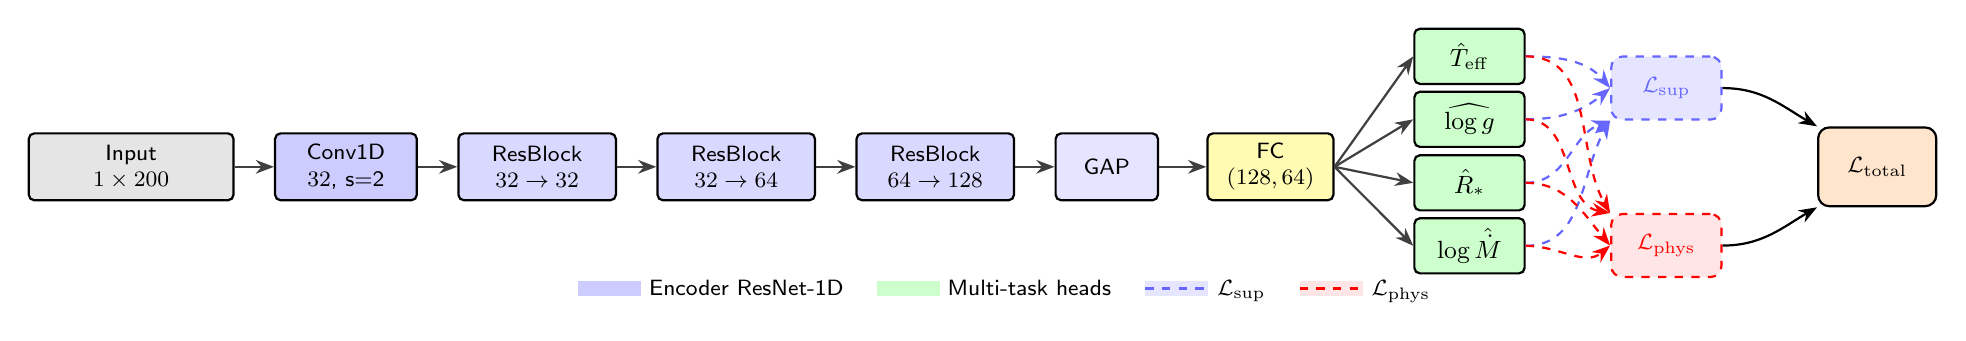
\begin{tikzpicture}[
    font=\sffamily\footnotesize,
    >=Stealth,
    box/.style={draw, thick, rounded corners=2pt, align=center, minimum height=0.85cm},
    input/.style={box, fill=gray!20, minimum width=2.6cm},
    conv/.style={box, fill=blue!20, minimum width=1.8cm},
    res/.style={box, fill=blue!15, minimum width=2cm},
    pool/.style={box, fill=blue!10, minimum width=1.3cm},
    fc/.style={box, fill=yellow!30, minimum width=1.6cm},
    head/.style={box, fill=green!20, minimum width=1.4cm, minimum height=0.7cm, font=\small},
    arrow/.style={->, thick, draw=gray!50!black},
    physarrow/.style={->, thick, red, dashed},
    dataarrow/.style={->, thick, blue!60, dashed}
]

% --- Encoder ---
\node[input] (in) {Input\\$1 \times 200$};
\node[conv, right=0.5cm of in] (c1) {Conv1D\\$32$, s=2};
\node[res, right=0.5cm of c1] (r1) {ResBlock\\$32 \to 32$};
\node[res, right=0.5cm of r1] (r2) {ResBlock\\$32 \to 64$};
\node[res, right=0.5cm of r2] (r3) {ResBlock\\$64 \to 128$};
\node[pool, right=0.5cm of r3] (gap) {GAP};
\node[fc, right=0.6cm of gap] (lat) {FC\\$(128, 64)$};

\draw[arrow] (in) -- (c1);
\draw[arrow] (c1) -- (r1);
\draw[arrow] (r1) -- (r2);
\draw[arrow] (r2) -- (r3);
\draw[arrow] (r3) -- (gap);
\draw[arrow] (gap) -- (lat);

% --- Heads ---
\node[head, above right=0.6cm and 1.0cm of lat] (teff) {$\hat{T}_{\rm eff}$};
\node[head, above right=-0.2cm and 1.0cm of lat] (logg) {$\widehat{\log g}$};
\node[head, below right=0.2cm and 1.0cm of lat] (mdot) {$\log\hat{\dot{M}}$};
\node[head, below right=-0.6cm and 1.0cm of lat] (rad) {$\hat{R}_{*}$};

\draw[arrow] (lat.east) -- (teff.west);
\draw[arrow] (lat.east) -- (logg.west);
\draw[arrow] (lat.east) -- (mdot.west);
\draw[arrow] (lat.east) -- (rad.west);

% --- Losses ---
\node[draw, thick, dashed, blue!60, fill=blue!10, rounded corners,
      minimum width=1.4cm, minimum height=0.8cm, align=center,
      right=3.5cm of lat, yshift=1.0cm] (data) {$\mathcal{L}_{\rm sup}$};

\node[draw, thick, dashed, red, fill=red!10, rounded corners,
      minimum width=1.4cm, minimum height=0.8cm, align=center,
      right=3.5cm of lat, yshift=-1.0cm] (phys) {$\mathcal{L}_{\rm phys}$};

% --- Total loss ---
\path (data.east) -- (phys.east) coordinate[midway] (midloss);
\node[draw, thick, fill=orange!20, rounded corners,
      minimum width=1.5cm, minimum height=1.0cm, align=center,
      right=1.2cm of midloss] (total) {$\mathcal{L}_{\rm total}$};

\draw[dataarrow] (teff.east) to[out=0, in=130] (data.west);
\draw[dataarrow] (logg.east) to[out=0, in=220] (data.west);
\draw[dataarrow] (mdot.east) to[out=0, in=240] (data.south west);
\draw[dataarrow] (rad.east) to[out=0, in=200] (data.south west);

\draw[physarrow] (teff.east) to[out=0, in=120] (phys.north west);
\draw[physarrow] (logg.east) to[out=0, in=170] (phys.north west);
\draw[physarrow] (mdot.east) to[out=0, in=220] (phys.west);
\draw[physarrow] (rad.east) to[out=0, in=130] (phys.west);

\draw[->, thick] (data.east) to[out=0, in=150] (total.north west);
\draw[->, thick] (phys.east) to[out=0, in=210] (total.south west);

% --- Leyenda ---
\node[anchor=north, yshift=-0.8cm] at ($(in.south)!0.5!(total.south)$) {
    \begin{tabular}{cccc}
    \tikz{\fill[blue!20] (0,0) rectangle (0.8,0.18);} Encoder ResNet-1D &
    \tikz{\fill[green!20] (0,0) rectangle (0.8,0.18);} Multi-task heads &
    \tikz{\fill[blue!10] (0,0) rectangle (0.8,0.18); \draw[thick, dashed, blue!60] (0,0.09) -- (0.8,0.09);} $\mathcal{L}_{\rm sup}$ &
    \tikz{\fill[red!10] (0,0) rectangle (0.8,0.18); \draw[thick, dashed, red] (0,0.09) -- (0.8,0.09);} $\mathcal{L}_{\rm phys}$
    \end{tabular}
};

\end{tikzpicture}
}
  \caption{Arquitectura ResNet-1D con cabezas multitarea y términos de pérdida. Las flechas continuas (grises) indican el flujo de \emph{forward pass}; las punteadas azules conectan las predicciones con $\mathcal{L}_{\mathrm{sup}}$ (pérdida supervisada); las punteadas rojas indican el cálculo del residuo físico (Ec.~\ref{eq:r_phys}) sobre las predicciones que alimenta $\mathcal{L}_{\mathrm{phys}}$.}
  \label{fig:modelo-full}
\end{figure*}

\paragraph{Cabezas de predicción multi-tarea.} Desde la representación latente $\mathbf{z} \in \mathbb{R}^{64}$, cada parámetro se predice mediante una cabeza independiente con arquitectura $\mathrm{Dense}(128) \rightarrow \mathrm{BN} \rightarrow \mathrm{Dropout}(0.3) \rightarrow \mathrm{Output}$. Los cuatro parámetros ($T_{\mathrm{eff}}$, $\log g$, $\log \dot{M}$, $R_{*}$) se predicen mediante salida lineal (regresión continua en espacio normalizado $[0,1]$). La grilla ISOSCELES discretiza $\log g$ en seis valores por construcción ($\mathcal{G} = \{3.15, 3.30, 3.45, 3.60, 3.75, 3.90\}$): las etiquetas sintéticas de validación y prueba viven exactamente sobre esos nodos. Por ello, al medir el rendimiento in-distribution sobre ISOSCELES proyectamos la predicción continua al nodo más cercano (\emph{snap}):
\begin{equation}
  \widehat{\log g}_{\mathrm{snap}} = \arg\min_{g_c \in \mathcal{G}} \left| \widehat{\log g} - g_c \right|,
  \label{eq:logg_snap}
\end{equation}
En la evaluación fuera de distribución sobre IACOB ---cuyas estrellas reales poseen $\log g$ continuo--- reportamos la predicción sin \emph{snap}, evitando introducir cuantización artificial e inflar el error para estrellas situadas entre nodos. Crucialmente, el \emph{snap} se aplica únicamente en la evaluación in-distribution; durante el entrenamiento, tanto $\mathcal{L}_{\mathrm{sup}}$ como $\mathcal{L}_{\mathrm{phys}}$ operan sobre el valor continuo $\widehat{\log g}$, preservando la diferenciabilidad end-to-end.

El número total de parámetros entrenables es $\approx 10^5$, lo que permite entrenamiento eficiente en hardware modesto.

\subsection{Función de pérdida compuesta}
\label{subsec:loss}

La función de pérdida total combina un término de supervisión estándar con una restricción física derivada de la prescripción autoconsistente de Figueroa-Tapia et al.~\cite{FigueroaTapia2026}.

\paragraph{Pérdida supervisada.} Todos los parámetros se predicen por regresión continua en espacio normalizado (Ec.~\ref{eq:minmax}), por lo que la pérdida supervisada es un MSE uniforme:
\begin{equation}
  \mathcal{L}_{\mathrm{sup}} = \frac{1}{4}\sum_{k \in \{T_{\mathrm{eff}}, \log g, \log \dot{M}, R_{*}\}} \left(\tilde{y}_k - \hat{\tilde{y}}_k\right)^2.
  \label{eq:l_sup}
\end{equation}

Dado que $\mathcal{L}_{\mathrm{sup}}$ opera enteramente en $[0,1]$, las contribuciones de los cuatro parámetros están en escalas comparables por construcción, evitando que el optimizador se sesgue hacia parámetros con rangos numéricos mayores (e.g.\ $T_{\mathrm{eff}} \sim 10^4$ vs.\ $\log g \sim 4$). En contraste, $\mathcal{L}_{\mathrm{phys}}$ debe evaluarse en espacio físico: las predicciones normalizadas $\hat{\tilde{y}}$ se desnormalizan antes de aplicar la prescripción CNO, garantizando que el residuo $r_{\mathrm{phys}}$ esté expresado en unidades físicas.

\paragraph{Pérdida física.} Para el término de penalización empleamos los valores centrales de la prescripción CNO (Ec.~\ref{eq:cno_uncert}):
\begin{equation}
  \log \dot{M}_{\mathrm{CNO}} = -20.74 + 1.44\log\left(\frac{R_{*}}{R_\odot}\right) - 3.85\log g + 16.81\log\left(\frac{T_{\mathrm{eff}}}{1000\,\mathrm{K}}\right).
  \label{eq:cno_loss}
\end{equation}
Las incertidumbres de los coeficientes (Ec.~\ref{eq:cno_uncert}) no se propagan al término de pérdida en este trabajo: tratarlas requeriría un esquema bayesiano o una función de pérdida con varianza no constante que dejamos como trabajo futuro. Esta decisión implica que $\mathcal{L}_{\mathrm{phys}}$ penaliza desviaciones respecto al valor central de la prescripción, asumiéndolo como verdad de referencia durante el entrenamiento.

Definimos el residuo físico para una predicción $\hat{\mathbf{y}}$ como:
\begin{equation}
  r_{\mathrm{phys}}(\hat{\mathbf{y}}) = \log \hat{\dot{M}} - \log \dot{M}_{\mathrm{CNO}}(\hat{T}_{\mathrm{eff}}, \widehat{\log g}, \hat{R}_{*}),
  \label{eq:r_phys}
\end{equation}
y la pérdida física como:
\begin{equation}
  \mathcal{L}_{\mathrm{phys}} = \frac{1}{N}\sum_{i=1}^{N} \left(r_{\mathrm{phys}}(\hat{\mathbf{y}}_i)\right)^2.
  \label{eq:l_phys}
\end{equation}

Empleamos un MSE sobre el residuo $r_{\mathrm{phys}}$ por su diferenciabilidad suave y porque penaliza con fuerza las violaciones grandes ---predicciones lejos de la variedad CNO, justo el régimen que buscamos corregir---; alternativas robustas (Huber, MAE o pérdidas por cuantiles sobre el residuo logarítmico), que atenúan la influencia de \emph{outliers}, son una extensión natural que dejamos como trabajo futuro.

La Figura~\ref{fig:concept_phys} esquematiza este cómputo: tres salidas de la red alimentan la prescripción CNO y el resultado se compara con $\log\hat{\dot{M}}$.

\begin{figure}[h]
  \centering
  \resizebox{0.9\columnwidth}{!}{%
  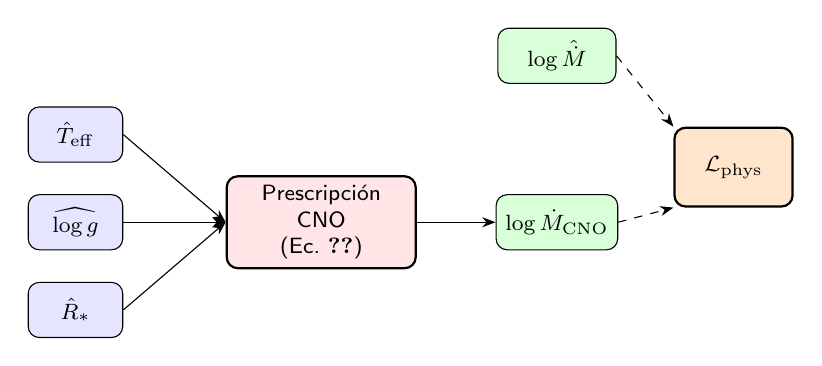
\begin{tikzpicture}[
      font=\sffamily\footnotesize,
      >=Stealth,
      node distance=0.4cm and 0.8cm,
      var/.style={draw, rounded corners, fill=blue!10, minimum width=1.2cm, minimum height=0.7cm},
      outnode/.style={draw, rounded corners, fill=green!15, minimum width=1.5cm, minimum height=0.7cm},
      eq/.style={draw, thick, rounded corners, fill=red!10, minimum width=2.4cm, minimum height=1cm, align=center}
  ]
    \node[var] (teff) {$\hat{T}_\mathrm{eff}$};
    \node[var, below=of teff] (logg) {$\widehat{\log g}$};
    \node[var, below=of logg] (rad) {$\hat{R}_*$};

    \node[eq, right=1.3cm of logg] (cno) {Prescripción\\CNO\\(Ec.~\ref{eq:cno_loss})};

    \node[outnode, right=1.0cm of cno] (mdot_pred) {$\log\dot{M}_\mathrm{CNO}$};
    \node[outnode, above=1.4cm of mdot_pred] (mdot_net) {$\log\hat{\dot{M}}$};
    \node[draw, thick, fill=orange!20, rounded corners, right=0.7cm of mdot_pred, yshift=0.7cm, minimum width=1.5cm, minimum height=1cm, align=center] (lphys) {$\mathcal{L}_\mathrm{phys}$};

    \draw[->] (teff.east) -- (cno.west);
    \draw[->] (logg.east) -- (cno.west);
    \draw[->] (rad.east) -- (cno.west);
    \draw[->] (cno.east) -- (mdot_pred.west);
    \draw[->, dashed] (mdot_net.east) -- (lphys.north west);
    \draw[->, dashed] (mdot_pred.east) -- (lphys.south west);
  \end{tikzpicture}}
  \caption{Esquema de $\mathcal{L}_\mathrm{phys}$ (Ec.~\ref{eq:l_phys}). Tres salidas de la red ($\hat{T}_\mathrm{eff}$, $\widehat{\log g}$, $\hat{R}_*$) se evalúan en la prescripción CNO (Ec.~\ref{eq:cno_loss}) y se comparan con $\log\hat{\dot{M}}$ mediante MSE (Ec.~\ref{eq:r_phys}). Flechas continuas: cómputo forward; punteadas: residuo. La restricción es diferenciable y no requiere etiquetas adicionales.}
  \label{fig:concept_phys}
\end{figure}

\paragraph{Pérdida total con activación diferida y rampa lineal.}
Para evitar que la restricción física domine prematuramente y ``atasque'' el entrenamiento en mínimos subóptimos, empleamos un scheduler bifásico para el peso $\lambda_{\mathrm{phys}}$:
\begin{equation}
  \lambda_{\mathrm{phys}}(e) =
  \begin{cases}
    0, & e < e_{\mathrm{delay}}, \\
    \lambda_{\max} \cdot \min\!\left(1,\, \frac{e - e_{\mathrm{delay}}}{e_{\mathrm{ramp}}}\right), & e \geq e_{\mathrm{delay}},
  \end{cases}
  \label{eq:lambda_schedule}
\end{equation}
donde $e$ es la época actual, $e_{\mathrm{delay}}$ el número de épocas de pre-entrenamiento supervisado puro (fase de delay, $\lambda_{\mathrm{phys}}=0$), $e_{\mathrm{ramp}}$ la duración de la rampa de activación lineal hasta alcanzar el peso final $\lambda_{\max}$. La distinción entre ambos parámetros es clave: $e_{\mathrm{delay}}$ controla \emph{cuándo} comienza a actuar la restricción física, mientras que $e_{\mathrm{ramp}}$ controla \emph{con qué velocidad} alcanza su peso objetivo.

La pérdida total es:
\begin{equation}
  \mathcal{L}_{\mathrm{total}} = \mathcal{L}_{\mathrm{sup}} + \lambda_{\mathrm{phys}}(e) \cdot \frac{\mathcal{L}_{\mathrm{phys}}}{\mathcal{L}_{\mathrm{phys}}^{\mathrm{ref}}},
  \label{eq:l_total}
\end{equation}
donde $\mathcal{L}_{\mathrm{phys}}^{\mathrm{ref}}$ es el MSE físico de las etiquetas sintéticas respecto a la prescripción CNO (Ec.~\ref{eq:cno_loss}), computado una sola vez sobre el conjunto de entrenamiento antes de iniciar el optimizador y tratado como constante durante todo el proceso. Este factor normaliza la escala del término físico haciéndola comparable con $\mathcal{L}_{\mathrm{sup}}$ independientemente del valor de $\lambda_{\max}$.

\paragraph{Interpretación conceptual de $\lambda_\mathrm{phys}$.}
Reconocemos una sutileza importante en la interpretación del peso $\lambda_\mathrm{phys}$. Tanto las etiquetas de $\log\dot{M}$ en ISOSCELES como la prescripción CNO de FT26 son construcciones teóricas que pueden discrepar sistemáticamente entre sí. En consecuencia, $\lambda_\mathrm{phys}$ no representa un balance puro entre ``datos observacionales'' y ``física'', sino entre dos prescripciones teóricas alternativas. Optamos por preferir FT26 como restricción suave por dos razones: (a) incorpora un tratamiento más reciente y autoconsistente de la dilución del flujo UV causada por líneas metálicas, corrigiendo la sobreestimación sistemática de $\dot{M}$ de prescripciones previas~\cite{FigueroaTapia2026}; y (b) ha sido validada externamente con $R^2 = 0.929$ sobre datos de ajuste. Cuantificamos la discrepancia entre ambas prescripciones sobre el conjunto sintético mediante $\mathcal{L}_\mathrm{phys}^\mathrm{ref}$, cuyo valor sobre el conjunto de entrenamiento es $\mathcal{L}_\mathrm{phys}^\mathrm{ref}=2.30$ (en dex$^2$ sobre $\log\dot{M}$); un valor alto de $\mathcal{L}_\mathrm{phys}^\mathrm{ref}$ indicaría que ambas teorías son inconsistentes sobre el dominio ISOSCELES y que un peso $\lambda_\mathrm{phys}$ grande sesgaría las predicciones hacia FT26 en detrimento del ajuste a las etiquetas sintéticas.

\paragraph{Balanceo entre términos de pérdida y alternativas adaptativas.}
La función de pérdida total combina dos términos que viven en espacios numéricos distintos: $\mathcal{L}_\mathrm{sup}$ se evalúa en el espacio normalizado $[0,1]$ (Ec.~\ref{eq:minmax}) sobre los cuatro parámetros, mientras que $\mathcal{L}_\mathrm{phys}$ se evalúa en espacio físico, como un MSE sobre el residuo de $\log\dot{M}$ medido en dex (Ec.~\ref{eq:r_phys}). Esta diferencia de unidades es la fuente de desbalance que motivó la observación de los revisores. Para documentarla, medimos las normas de los gradientes de cada término respecto a los parámetros del encoder compartido $\theta$ sobre un \emph{batch} real de $2048$ espectros (Tabla~\ref{tab:grad}). En el instante en que la rampa activa la física ---con la red supervisada ya convergida--- $\lVert\nabla_\theta\mathcal{L}_\mathrm{phys}\rVert$ supera a $\lVert\nabla_\theta\mathcal{L}_\mathrm{sup}\rVert$ por un factor ${\sim}190$ (más de dos órdenes de magnitud): sumar ambos términos sin tratamiento haría que el paso del optimizador estuviese dominado casi por completo por la física, suprimiendo el ajuste espectral. Es importante notar que la similitud coseno entre ambos gradientes es de sólo $+0.11$: los términos son casi ortogonales, no antagónicos. El conflicto es por tanto de \emph{magnitud} y no de \emph{dirección}, lo que implica que un único peso escalar $\lambda_\mathrm{phys}$ es suficiente para balancearlos, sin necesidad de cirugía de gradientes. Un desbalance secundario, de menor orden, proviene de la disparidad entre los coeficientes de la prescripción CNO (de $1.44$ a $16.81$), que produce gradientes de magnitud desigual respecto a $\hat{T}_\mathrm{eff}$, $\widehat{\log g}$ y $\hat{R}_*$.

\begin{table}[ht]
  \caption{Normas de los gradientes de cada término de pérdida respecto al
    encoder compartido $\theta$, sobre un \emph{batch} de $2048$ espectros
    sintéticos. El desbalance dominante es de \emph{magnitud} (${\sim}190\times$
    al activarse la física) y persiste tras la normalización por
    $\mathcal{L}_\mathrm{phys}^\mathrm{ref}$ (${\sim}83\times$); la similitud
    coseno cercana a cero confirma que los gradientes son casi ortogonales. La
    última fila muestra el peso $w_\mathrm{phys}$ que iguala ambas normas, que es
    el que GradNorm aprende de forma adaptativa (§\ref{subsec:gradnorm}).}
  \label{tab:grad}
  \small
  \setlength{\tabcolsep}{4pt}
  \begin{tabular}{@{}l c c c c@{}}
    \toprule
    & $\lVert\nabla\mathcal{L}_\mathrm{sup}\rVert$
    & $\lVert\nabla\mathcal{L}_\mathrm{phys}\rVert$
    & razón
    & $\cos$ \\
    \midrule
    Inicialización & $0.20$ & $19.9$ & $98\times$ & $+0.52$ \\
    Activación física & $1.74$ & $333$ & $192\times$ & $+0.11$ \\
    \;\;tras $\div\,\mathcal{L}_\mathrm{phys}^\mathrm{ref}$ & $1.74$ & $145$ & $83\times$ & $+0.11$ \\
    \;\;con GradNorm ($w_\mathrm{phys}{=}0.012$) & $1.74$ & $1.74$ & $\mathbf{1.0\times}$ & $+0.11$ \\
    \bottomrule
  \end{tabular}
\end{table}

Frente a este desbalance adoptamos, en la configuración principal de $\lambda_\mathrm{phys}$ fijo, un conjunto de mitigaciones estáticas. Primero, la normalización Min-Max (Ec.~\ref{eq:minmax}) garantiza que los cuatro parámetros contribuyan a $\mathcal{L}_\mathrm{sup}$ en escalas comparables, eliminando el sesgo trivial hacia parámetros con rangos numéricos mayores (e.g.\ $T_\mathrm{eff}\sim 10^4$ frente a $\log g\sim 4$). Segundo, la división por $\mathcal{L}_\mathrm{phys}^\mathrm{ref}$ (Ec.~\ref{eq:l_total}) ---un factor constante computado una sola vez sobre las etiquetas sintéticas--- lleva el \emph{valor} del término físico a una escala de referencia $\mathcal{O}(1)$ independiente de las unidades de $\log\dot{M}$, dando a $\lambda_\mathrm{phys}$ una interpretación directa como peso relativo. Conviene precisar que esta normalización reescala el \emph{valor} de la pérdida, no la \emph{norma} de su gradiente: como muestra la Tabla~\ref{tab:grad}, reduce el desbalance de gradientes de ${\sim}190\times$ a ${\sim}83\times$, pero no lo elimina. El balance efectivo restante lo fijan tres mecanismos complementarios: (i)~la activación diferida y la rampa lineal de $\lambda_\mathrm{phys}$ (Ec.~\ref{eq:lambda_schedule}), que introducen la física gradualmente sobre una red ya convergida; (ii)~el recorte global de norma de gradiente ($\lVert g\rVert\le 1$), que acota cada paso con independencia de la magnitud cruda del término físico; y (iii)~el valor $\lambda_\mathrm{phys}=0.25$ seleccionado por búsqueda en grilla (§\ref{subsec:training}). Con dicho valor, la contribución efectiva de la física al gradiente compartido sigue siendo ${\sim}20\times$ la supervisada en el instante de activación; este dominio es deliberado ---la restricción está pensada para reconfigurar el comportamiento fuera de distribución--- y su costo, una degradación controlada del MAE in-distribution, se cuantifica en los resultados.

Como los gradientes son casi ortogonales (Tabla~\ref{tab:grad}), no recurrimos a métodos de proyección de gradientes (tipo PCGrad), pensados para gradientes antagónicos: el conflicto es de magnitud, no de dirección. Ahora bien, ese desbalance residual de magnitud (${\sim}83\times$) implica que \emph{ningún} $\lambda_\mathrm{phys}$ fijo iguala las normas de los gradientes de ambos términos. Para abordar este punto de forma directa ---y responder a la observación de los revisores sobre el escalado de gradientes--- implementamos además el balanceo adaptativo GradNorm~\cite{Chen2018GradNorm}, que reemplaza el escalar fijo por un peso $w_\mathrm{phys}$ actualizado en cada paso de modo que las normas de los gradientes de $\mathcal{L}_\mathrm{sup}$ y $\mathcal{L}_\mathrm{phys}$ respecto al encoder compartido se igualen, moduladas por la tasa de aprendizaje relativa de cada término (parámetro de asimetría $\alpha=1.5$). A diferencia de $\lambda_\mathrm{phys}$, GradNorm no introduce un peso que ajustar a mano: el balance se determina solo. Reportamos esta variante junto a las configuraciones de $\lambda$ fijo en §\ref{subsec:gradnorm}, donde mostramos que (a)~conduce la razón de gradientes de ${\sim}83\times$ a ${\sim}1\times$ con un peso aprendido $w_\mathrm{phys}\!\approx\!0.01$, y (b)~la corrección fuera de distribución \emph{persiste}, lo que confirma que el efecto del término físico es robusto al mecanismo de balanceo y no un artefacto de un $\lambda$ ajustado manualmente. Mantenemos $\lambda_\mathrm{phys}=0.25$ como configuración principal por comparabilidad con el barrido de sensibilidad (§\ref{subsec:training}), y reservamos la ponderación por incertidumbre como extensión para versiones con múltiples restricciones físicas.

La diferenciabilidad de $\mathcal{L}_{\mathrm{phys}}$ respecto a todas las salidas predichas permite retropropagación directa mediante autodiferenciación, sin requerir información adicional del dominio observacional.

\subsection{Estrategias de entrenamiento}
\label{subsec:training}

Evaluamos dos configuraciones principales que permiten aislar el efecto de la restricción física:

\begin{description}
  \item[\textbf{Baseline}] Entrenamiento supervisado puro con $\lambda_{\mathrm{phys}} \equiv 0$. Sirve como referencia para cuantificar la degradación por brecha sintética.

  \item[\textbf{PGNN (Physics-Guided Neural Network)}] Entrenamiento con la función de pérdida compuesta de la Ec.~\eqref{eq:l_total}, incluyendo el término físico con rampa lineal de $\lambda_{\mathrm{phys}}$. Se evalúan tres variantes de ablación:
  \begin{enumerate}
    \item \emph{ft} (\emph{fine-tuning}) sobre el Baseline ya entrenado: $e_{\mathrm{delay}}=0$, $e_{\mathrm{ramp}}=10$. Al partir de pesos supervisados ya convergidos, la fase de delay es innecesaria y la rampa actúa desde la primera época.
    \item \emph{scratch} (\emph{from scratch}) en dos fases: $e_{\mathrm{delay}}=10$, $e_{\mathrm{ramp}}=20$. El delay garantiza que el encoder aprenda primero representaciones espectrales estables antes de que la restricción física comience a actuar.
    \item \emph{domain}: idéntico scheduler a \emph{scratch}, con penalizaciones de dominio adicionales (peso $w_{\mathrm{dom}}=0.1$) que castigan predicciones físicamente inadmisibles, $R_* < 0$ (radio negativo) y $\log \dot{M} > 0$, imponiendo el dominio físico directamente en la pérdida.
  \end{enumerate}

\end{description}
  
Como segundo eje de ablación, cada estrategia se entrena en dos modos según la \emph{fuente} de la restricción física: \emph{synth-only}, con $\mathcal{L}_\mathrm{phys}$ evaluada únicamente sobre espectros sintéticos; y \emph{+obs}, que tras completarse la rampa añade un término $w_\mathrm{obs}\,\mathcal{L}_\mathrm{phys}$ evaluado sobre los espectros observados (IACOB, $184$; UVES~POP~O, $12$) \emph{sin usar sus etiquetas}. Fijamos $w_\mathrm{obs}=0.01$, un orden de magnitud por debajo de $\lambda_\mathrm{phys}$: como el término se activa tras la rampa ---con la red ya convergida y satisfaciendo aproximadamente la prescripción CNO sobre el dominio observado--- su contribución resultante es ${\sim}8\%$ de $\mathcal{L}_\mathrm{sup}$. El valor conservador es deliberado: al carecer este término de supervisión, un peso elevado arriesgaría colapsar las predicciones hacia la variedad CNO en detrimento del ajuste espectral. El modo \emph{+obs} permite que la red ajuste su consistencia física directamente en el dominio observacional mediante la única restricción no supervisada disponible: la prescripción CNO. El cruce de ambos ejes produce $6$ configuraciones PGNN ($3$ estrategias $\times$ \{synth-only, +obs\}) que, junto al Baseline, conforman las $7$ configuraciones reportadas. En conjunto, las ablaciones aíslan el efecto de: (a)~el término físico, (b)~la estrategia de activación (diferida vs.\ fine-tuning), (c)~las penalizaciones de dominio, y (d)~la inclusión de física observacional.

Todos los modelos se entrenan con optimizador Adam ($\beta_1=0.9$, $\beta_2=0.999$), \emph{learning rate} inicial $5\times10^{-4}$, con reducción por plato ($\times 0.5$, paciencia 4--5) y \emph{early stopping} (paciencia 8--10, restauración de mejores pesos). El tamaño de \emph{batch} es $2048$ y se entrena hasta un máximo de $200$ épocas. Se aplica recorte de norma de gradiente máxima $1.0$ y precisión mixta (con $\mathcal{L}_\mathrm{phys}$ evaluada en \texttt{float32}). En las variantes PGNN, el \emph{checkpoint} final se fuerza al completarse la rampa (\emph{reset-after-ramp}), de modo que el modelo evaluado siempre incorpora la física y no el mínimo puramente supervisado que el \emph{early stopping} restauraría. El \emph{learning rate} se mantiene idéntico en todas las variantes para garantizar que las diferencias observadas se deban exclusivamente a la estrategia de activación, la fuente de la física o las penalizaciones de dominio.

\paragraph{Selección de $\lambda_{\mathrm{phys}}$.} El peso $\lambda_{\mathrm{phys}}$ se elige mediante un barrido $\lambda_{\mathrm{phys}} \in \{0.05, 0.10, 0.20, 0.25, 0.30, 0.50\}$ aplicado a cada estrategia con el scheduler y el resto de hiperparámetros fijos. Fijamos $\lambda_{\mathrm{phys}}=0.25$ \emph{a priori}, como un valor moderado: su elección \emph{no} se optimiza sobre los conjuntos observacionales. El barrido sobre IACOB (Tabla~\ref{tab:sweep}) es un análisis de sensibilidad \emph{a posteriori} ---que muestra que el error OOD es plano frente a $\lambda_{\mathrm{phys}}$--- y no un criterio de selección, evitando el ajuste de hiperparámetros sobre datos de evaluación. El costo in-distribution, medible sobre la validación sintética, crece monótonamente con $\lambda_{\mathrm{phys}}$, lo que respalda mantener un valor moderado. Los parámetros del scheduler ($e_{\mathrm{delay}}$, $e_{\mathrm{ramp}}$) se determinaron a partir de curvas de convergencia preliminares sobre el conjunto de validación, asegurando que la restricción física se active solo una vez que $\mathcal{L}_{\mathrm{sup}}$ se ha estabilizado. Para garantizar reproducibilidad estadística, los experimentos principales se ejecutan con cinco semillas aleatorias independientes (\{$42, 123, 2026, 7, 2024$\}); el barrido de sensibilidad de $\lambda_{\mathrm{phys}}$ (Tabla~\ref{tab:sweep}) se reporta con las tres primeras. La Figura~\ref{fig:training} ilustra la dinámica de entrenamiento bifásica resultante.

\begin{figure}[t]
  \centering
  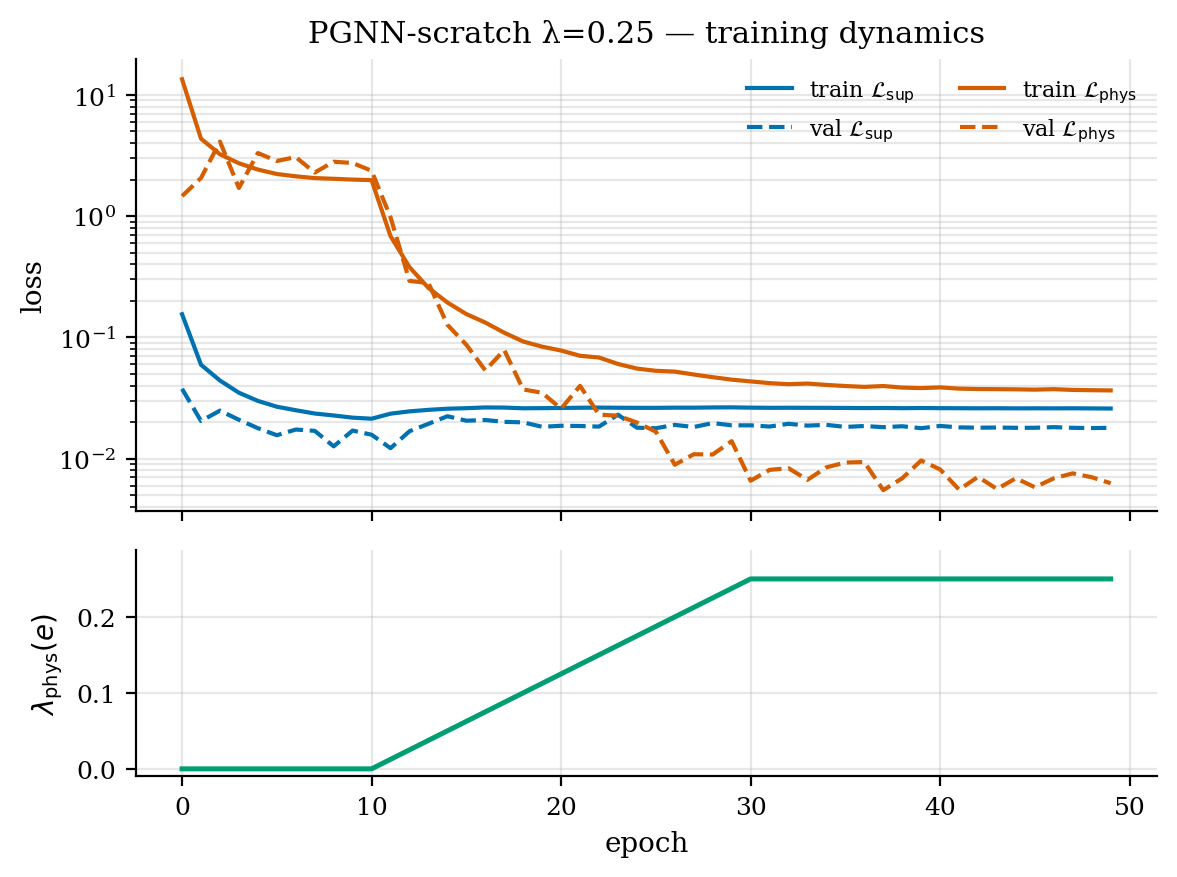
\includegraphics[width=\columnwidth]{fig5_training_curves.png}
  \caption{Dinámica de entrenamiento de PGNN-\emph{scratch}
  ($\lambda_\mathrm{phys}=0.25$). Arriba: pérdidas supervisada
  ($\mathcal{L}_\mathrm{sup}$) y física ($\mathcal{L}_\mathrm{phys}$), entrenamiento
  y validación, por época. Abajo: el peso $\lambda_\mathrm{phys}(e)$ con su fase de
  \emph{delay} ($e<e_\mathrm{delay}=10$) y rampa lineal (Ec.~\ref{eq:lambda_schedule}).
  Al activarse la física, $\mathcal{L}_\mathrm{phys}$ cae dos órdenes de magnitud sin
  degradar $\mathcal{L}_\mathrm{sup}$: la restricción no desestabiliza el ajuste
  espectral.}
  \label{fig:training}
\end{figure}

\subsection{Protocolo de validación y métricas}
\label{subsec:protocolo}

\paragraph{Partición de datos.}
El conjunto sintético ISOSCELES (subconjunto O, $33\,444$ espectros) se divide
en 80\% entrenamiento, 10\% validación y 10\% prueba mediante partición aleatoria.
Los conjuntos observacionales (UVES~POP e IACOB, descritos en
\S\ref{subsec:datos}) se reservan para evaluación
\emph{out-of-distribution} (OOD): sus \emph{etiquetas} nunca intervienen en el
entrenamiento ni en la selección de hiperparámetros. La configuración principal
(\emph{synth-only}) no observa ningún espectro real, por lo que su evaluación OOD
es estrictamente inductiva; las variantes \emph{+obs}
(§\ref{subsec:training}) usan los espectros observados \emph{sin etiqueta} en la
restricción física ---un uso transductivo de las entradas que tenemos en cuenta al
interpretar sus métricas.

\paragraph{Métricas.}
Organizamos las métricas en tres niveles de evaluación, de menor a mayor
exigencia:

\begin{enumerate}
  \item \textbf{Rendimiento in-distribution} (prueba sintética): MAE y RMSE
    por parámetro. Establece el techo de rendimiento del modelo en ausencia de
    brecha de dominio.

  \item \textbf{Coherencia distribucional OOD} (UVES~POP): distancia de
    Wasserstein-1 ($W_1$) entre la distribución \emph{real} de parámetros del
    conjunto sintético de prueba (etiquetas ISOSCELES) y la distribución
    \emph{predicha} sobre UVES~POP. Tomamos como referencia las etiquetas
    sintéticas reales ---y no las predicciones del modelo sobre el conjunto
    sintético--- para que la métrica no pueda minimizarse trivialmente colapsando
    ambas distribuciones predichas a una misma banda. $W_1$ cuantifica
    el desplazamiento promedio entre distribuciones en unidades del parámetro, capturando la magnitud de la discrepancia y no solo su significancia estadística

  \item \textbf{Error OOD contra etiquetas reales} (IACOB): MAE, RMSE y sesgo
    ($\bar{\delta} = \overline{\hat{y} - y}$) por parámetro contra los valores
    de literatura. $T_{\mathrm{eff}}$ y $\log g$ se evalúan contra ambos
    catálogos; $R_*$ se evalúa únicamente contra Holgado et
    al.~\cite{Holgado2025}, que proporciona estimaciones directas.
\end{enumerate}

Adicionalmente reportamos dos métricas transversales:

\begin{itemize}
  \item \textbf{Consistencia física:} $\mathcal{L}_{\mathrm{phys}}$ (Ec.~\ref{eq:l_phys}) promediada por separado en el conjunto sintético de prueba y en cada conjunto observacional. Dado que la prescripción CNO es el mismo término utilizado durante el entrenamiento del modelo PGNN, esta métrica cuantifica la coherencia interna de las predicciones y no constituye una validación independiente de $\log \dot{M}$; y no la interpretamos como tal.

  \item \textbf{Brecha de dominio:}
    $\Delta_k = \mathrm{MAE}_k^{\mathrm{IACOB}} -
    \mathrm{MAE}_k^{\mathrm{synth}}$ por parámetro $k$. Una brecha positiva
    indica degradación al pasar de datos sintéticos a observados; la hipótesis central predice que PGNN reducirá $\Delta_k$ respecto al Baseline.

  \item \textbf{Tasa de predicciones fuera de rango físico:} porcentaje de
    predicciones sobre IACOB que caen fuera de los rangos de validez FT26 para
    estrellas O ($T_{\mathrm{eff}}\in[30\,000,50\,000]$\,K, $\log g\in[2.9,4.3]$,
    $R_*\in[7,70]\,R_\odot$), reportado por parámetro. A diferencia de
    $\mathcal{L}_{\mathrm{phys}}$, no depende de la prescripción CNO ni de
    etiquetas: sólo verifica si las predicciones respetan los límites físicos del
    régimen O, por lo que constituye una comprobación de admisibilidad independiente.
\end{itemize}
    
\paragraph{Baselines.}
El \textbf{Baseline} ($\lambda_{\mathrm{phys}} \equiv 0$) cuantifica la
degradación causada por la brecha sintética sin mitigación. La variante PGNN
\emph{from-scratch}~(ii) sirve como control adicional: durante su fase de
delay ($e < e_{\mathrm{delay}}$, donde $\lambda_{\mathrm{phys}} = 0$), es
funcionalmente idéntica al Baseline pero con el mismo scheduler de
\emph{learning rate}. Comparar ambos verifica que la arquitectura de
entrenamiento bifásico no introduce ventajas artificiales, aislando el efecto neto
del término físico.


\section{Resultados}
\label{sec:resultados}

Reportamos las siete configuraciones descritas en §\ref{subsec:training}: el
\textbf{Baseline} supervisado y las seis variantes PGNN que cruzan la estrategia
de activación (\emph{ft}, \emph{scratch}, \emph{domain}) con la fuente de la
restricción física (\emph{synth-only}, \emph{+obs}), todas con
$\lambda_\mathrm{phys}=0.25$. Cada celda es la media $\pm$ desviación estándar
sobre las cinco semillas $\{42, 123, 2026, 7, 2024\}$. La evaluación sigue el protocolo de
tres niveles de §\ref{subsec:protocolo}; recordamos que $\log g$ se proyecta a la
grilla (\emph{snap}) sólo en la evaluación in-distribution sobre ISOSCELES, no en
IACOB.

\subsection{Rendimiento in-distribution (ISOSCELES)}

La Tabla~\ref{tab:iso} establece el techo de rendimiento en ausencia de brecha de
dominio. El Baseline alcanza el menor error en los cuatro parámetros
($T_\mathrm{eff}$: $657$\,K; $\log g$: $0.013$; $\log\dot{M}$: $0.24$;
$R_*$: $0.59\,R_\odot$). Todas las variantes PGNN degradan el ajuste sintético: el
MAE de $T_\mathrm{eff}$ se duplica ($\sim$1300--1540\,K), el de $\log g$ se
sextuplica ($\sim$0.07--0.09) y el de $\log\dot{M}$ se triplica ($\sim$0.74--0.78).
Esta degradación es esperada y deliberada: la restricción física reconfigura el
modelo para priorizar la consistencia fuera de distribución a costa del ajuste
in-distribution. La magnitud del costo es estable entre estrategias, lo que indica
que proviene del término físico en sí y no de la estrategia de activación.

\begin{table}[htbp]
  \caption{Nivel 1 --- MAE in-distribution sobre la prueba sintética ISOSCELES
  (menor es mejor). $T_\mathrm{eff}$ en K, $R_*$ en $R_\odot$,
  $\log g$ y $\log\dot{M}$ adimensionales.}
  \label{tab:iso}
  \scriptsize
  \setlength{\tabcolsep}{3pt}
  \begin{tabular}{lrrrr}
    \toprule
    Config. & $T_\mathrm{eff}$ & $\log g$ & $\log\dot{M}$ & $R_*$ \\
    \midrule
    Baseline          & \textbf{660}$\pm$250 & \textbf{0.013}$\pm$0.011 & \textbf{0.232}$\pm$0.055 & \textbf{0.51}$\pm$0.26 \\
    \emph{ft}         & 1371$\pm$47  & 0.074$\pm$0.003 & 0.755$\pm$0.014 & 0.85$\pm$0.05 \\
    \emph{scratch}    & 1526$\pm$37  & 0.080$\pm$0.004 & 0.750$\pm$0.008 & 0.92$\pm$0.04 \\
    \emph{domain}     & 1511$\pm$70  & 0.079$\pm$0.003 & 0.744$\pm$0.009 & 0.92$\pm$0.01 \\
    \emph{ft}+obs     & 1474$\pm$231 & 0.080$\pm$0.013 & 0.780$\pm$0.017 & 1.02$\pm$0.10 \\
    \emph{scratch}+obs& 1353$\pm$45  & 0.087$\pm$0.003 & 0.754$\pm$0.009 & 0.97$\pm$0.05 \\
    \emph{domain}+obs & 1283$\pm$84  & 0.087$\pm$0.002 & 0.750$\pm$0.023 & 0.99$\pm$0.04 \\
    \bottomrule
  \end{tabular}
\end{table}

\subsection{Error fuera de distribución contra literatura (IACOB)}

La Tabla~\ref{tab:iacob} es el resultado central. Sobre las 184 estrellas IACOB
reales, el Baseline exhibe un error catastrófico y de alta varianza:
$\mathrm{MAE}(T_\mathrm{eff})=10\,343$\,K con un sesgo de
$+10\,091$\,K ---el modelo \emph{sobreestima} sistemáticamente la temperatura en
$\sim$10\,kK---, $\mathrm{MAE}(\log g)=0.40$ con sesgo $+0.27$, y
$\mathrm{MAE}(R_*)=4.6\,R_\odot$ con sesgo $-3.8\,R_\odot$ (subestima el radio).

Todas las variantes PGNN colapsan este error a una banda estrecha y casi
independiente de la semilla: $\mathrm{MAE}(T_\mathrm{eff})\!\approx\!3460$--$3730$\,K
(reducción del $\sim$66\%), $\mathrm{MAE}(\log g)\!\approx\!0.25$--$0.26$
($\sim$37\%) y $\mathrm{MAE}(R_*)\!\approx\!3.5$--$3.6\,R_\odot$ ($\sim$25\%).
Más relevante que el MAE es la \emph{corrección del sesgo}: el sesgo de
$T_\mathrm{eff}$ cae de $+10$\,kK a $\sim\!-2.3$\,kK, el de $\log g$ de $+0.27$ a
$\sim\!-0.10$ y el de $R_*$ de $-3.8$ a $\sim\!0$. La restricción física no sólo
reduce la dispersión sino que reubica las predicciones dentro del régimen físico,
confirmando la hipótesis central para $T_\mathrm{eff}$, $\log g$ y $R_*$. La mejor
configuración en $T_\mathrm{eff}$ es \emph{ft} ($3460$\,K); las diferencias entre
estrategias de activación y entre \emph{synth-only} y \emph{+obs} son de segundo
orden frente al salto respecto al Baseline. La Figura~\ref{fig:scatter} visualiza
esta corrección: las predicciones del Baseline (rojo) se alejan de la recta 1:1
---$T_\mathrm{eff}$ y $\log g$ sobreestimados, $R_*$ subestimado--- mientras que
PGNN (azul) las recentra sobre la diagonal y dentro del rango físico (banda verde).

\begin{table}[htbp]
  \caption{Nivel 3 --- Error fuera de distribución sobre IACOB contra etiquetas de
  literatura. MAE (menor es mejor) y sesgo $\bar{\delta}=\overline{\hat{y}-y}$
  (más cercano a 0 es mejor). $T_\mathrm{eff}$ y $\log g$ sobre 184 estrellas;
  $R_*$ sobre las 148 con radio disponible.}
  \label{tab:iacob}
  \scriptsize
  \setlength{\tabcolsep}{2.5pt}
  \begin{tabular}{lrrrrrr}
    \toprule
    & \multicolumn{2}{c}{$T_\mathrm{eff}$ [K]} & \multicolumn{2}{c}{$\log g$} & \multicolumn{2}{c}{$R_*$ [$R_\odot$]} \\
    \cmidrule(lr){2-3}\cmidrule(lr){4-5}\cmidrule(lr){6-7}
    Config. & MAE & sesgo & MAE & sesgo & MAE & sesgo \\
    \midrule
    Baseline           & 10343$\pm$2748 & $+10091$ & 0.40$\pm$0.09 & $+0.27$ & 4.63$\pm$0.15 & $-3.77$ \\
    \emph{ft}          & \textbf{3460}$\pm$85  & $-2318$ & \textbf{0.25} & $-0.09$ & \textbf{3.46} & $-0.07$ \\
    \emph{scratch}     & 3732$\pm$159 & $-2614$ & 0.26 & $-0.11$ & 3.56 & $+0.48$ \\
    \emph{domain}      & 3584$\pm$179 & $-2452$ & 0.26 & $-0.10$ & 3.50 & $+0.17$ \\
    \emph{ft}+obs      & 3631$\pm$164 & $-2651$ & 0.26 & $-0.11$ & 3.56 & $+0.43$ \\
    \emph{scratch}+obs & 3635$\pm$103 & $-2308$ & 0.25 & $-0.10$ & 3.58 & $+0.42$ \\
    \emph{domain}+obs  & 3550$\pm$156 & $-2407$ & 0.26 & $-0.11$ & 3.61 & $+0.36$ \\
    \bottomrule
  \end{tabular}
\end{table}

\begin{figure*}[ht]
  \centering
  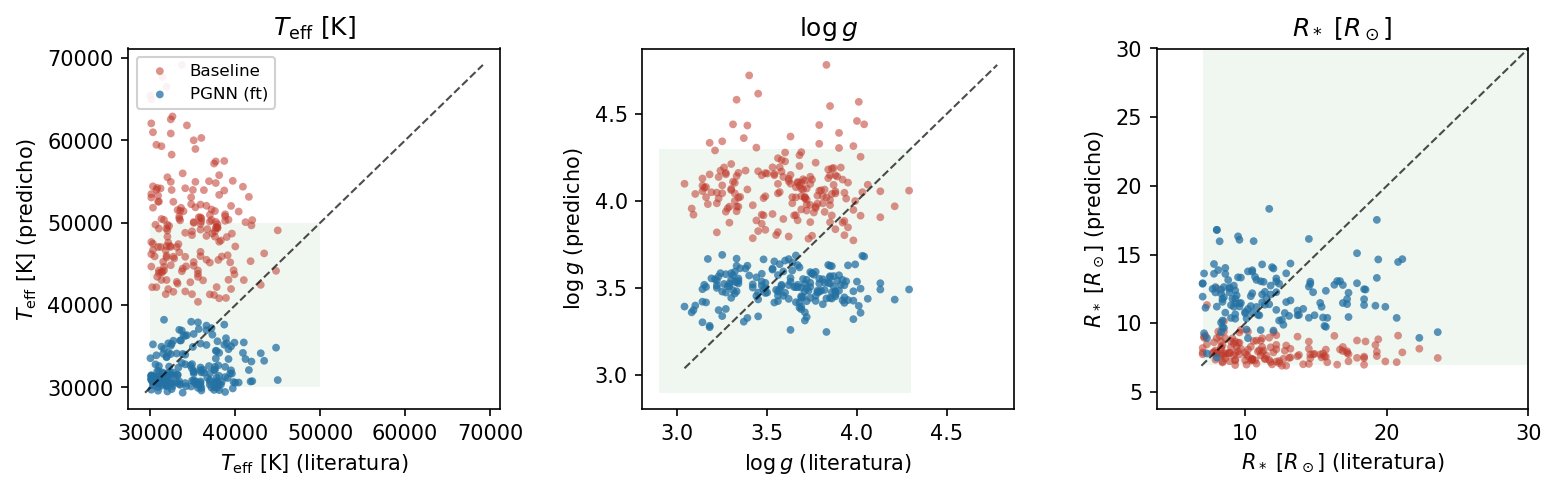
\includegraphics[width=0.8\textwidth]{fig_iacob_scatter.png}
  \caption{Predicción vs.\ literatura sobre IACOB (semilla 42) para
  $T_\mathrm{eff}$, $\log g$ y $R_*$. Baseline (rojo) frente a PGNN-\emph{ft}
  (azul); línea discontinua = identidad 1:1. La banda verde marca la región
  físicamente admisible (rango de validez FT26 del parámetro: $\log g\in[2.9,4.3]$,
  $R_*\in[7,70]\,R_\odot$). El Baseline sobreestima $T_\mathrm{eff}$ y $\log g$ y
  subestima $R_*$; la restricción física recentra las predicciones sobre la diagonal
  y dentro del régimen físico.}
  \label{fig:scatter}
\end{figure*}

\subsection{Coherencia distribucional (UVES~POP)}

La Tabla~\ref{tab:w1} reporta la distancia de Wasserstein-1 entre la distribución
real de parámetros de la prueba sintética (etiquetas ISOSCELES) y la predicha sobre
las 12 estrellas O de UVES~POP (sin etiquetas). El patrón refuerza el de IACOB para
$T_\mathrm{eff}$: $W_1$ cae de ${\sim}7900$\,K (Baseline) a $\sim$2100--2500\,K en todas
las variantes PGNN. Para $\log g$ la mejora es consistente aunque menor
($0.31\to0.12$--$0.17$). En cambio, $\log\dot{M}$ \emph{empeora}
($0.67\to0.91$--$1.01$) y $R_*$ muestra resultados mixtos (mejor con \emph{domain},
$3.04\to2.02$; peor con \emph{scratch}, $3.04\to3.39$). Discutimos estos dos casos
de fallo en §\ref{sec:discusion}. La Figura~\ref{fig:w1hist} muestra las
distribuciones predichas completas frente a la referencia sintética.

\begin{table}[htbp]
  \caption{Nivel 2 --- Distancia de Wasserstein-1 entre la distribución real de
  parámetros de la prueba sintética (etiquetas ISOSCELES) y la predicha sobre
  UVES~POP~O (sin etiquetas; menor es mejor). Unidades del parámetro.}
  \label{tab:w1}
  \scriptsize
  \setlength{\tabcolsep}{4pt}
  \begin{tabular}{lrrrr}
    \toprule
    Config. & $T_\mathrm{eff}$ & $\log g$ & $\log\dot{M}$ & $R_*$ \\
    \midrule
    Baseline           & 7928$\pm$2020 & 0.312 & \textbf{0.671} & 3.044 \\
    \emph{ft}          & \textbf{2122}$\pm$130 & 0.168 & 0.950 & 2.967 \\
    \emph{scratch}     & 2430$\pm$428  & 0.173 & 0.955 & 3.390 \\
    \emph{domain}      & 2382$\pm$420  & \textbf{0.121} & 0.912 & \textbf{2.020} \\
    \emph{ft}+obs      & 2404$\pm$436  & 0.173 & 0.957 & 3.042 \\
    \emph{scratch}+obs & 2493$\pm$915  & 0.159 & 0.982 & 3.156 \\
    \emph{domain}+obs  & 2413$\pm$461  & 0.167 & 1.011 & 2.938 \\
    \bottomrule
  \end{tabular}
\end{table}

\begin{figure}[htbp]
  \centering
  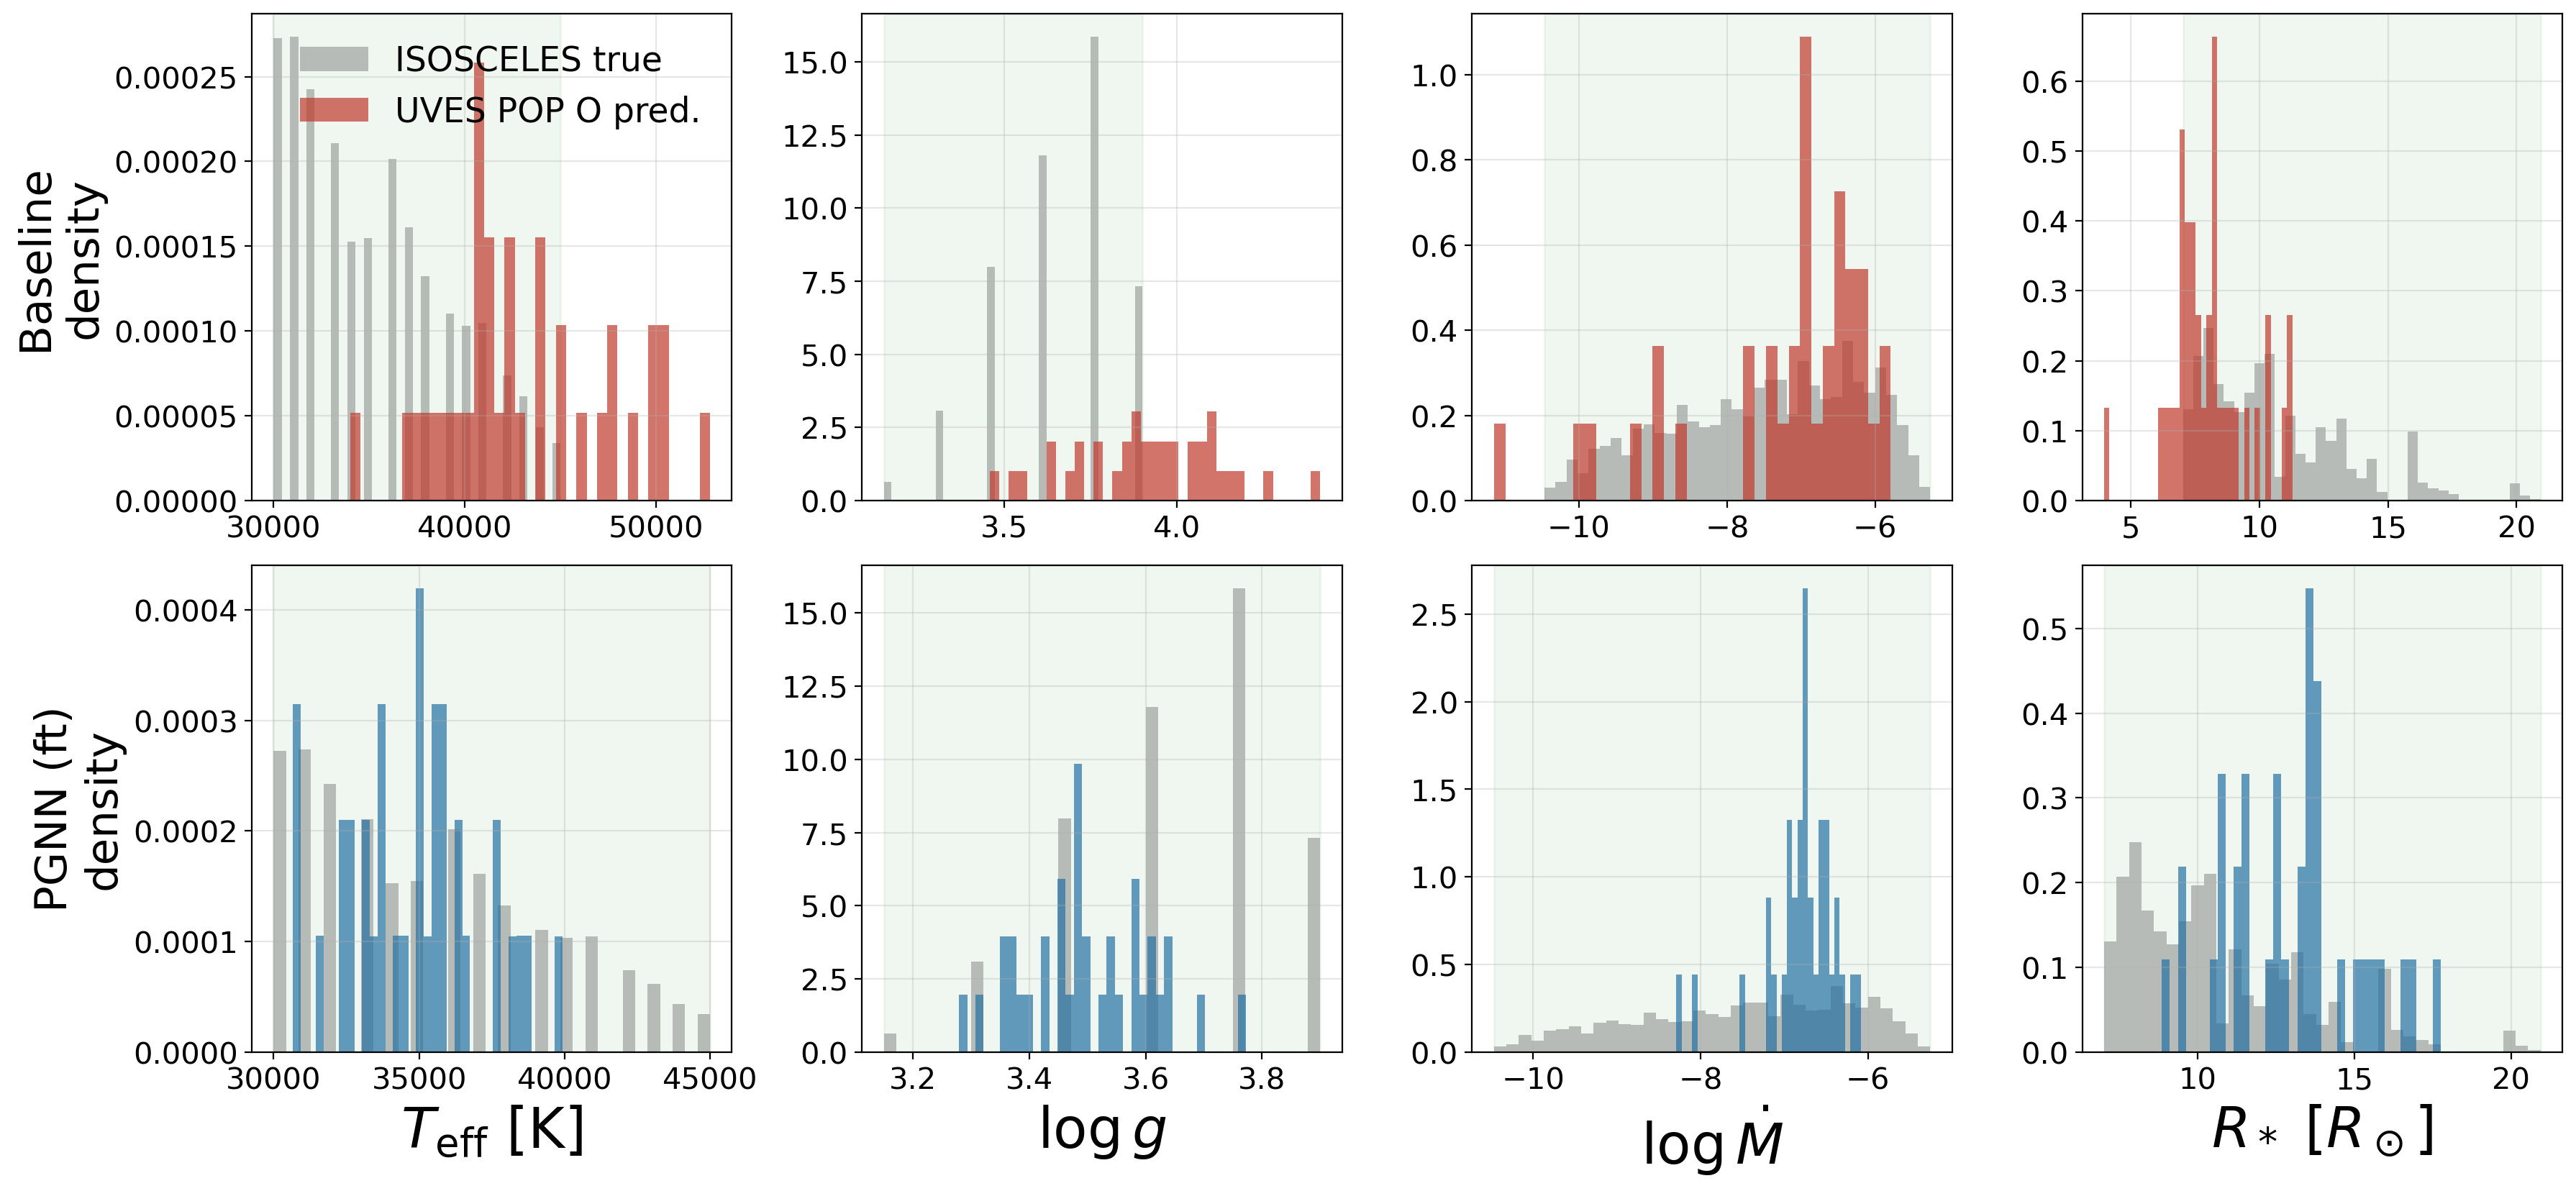
\includegraphics[width=\columnwidth]{fig9_uvespopO_histograms.png}
  \caption{Distribuciones de parámetros predichas sobre las 12 estrellas O de
  UVES~POP (color) frente a la distribución real de las etiquetas ISOSCELES (gris),
  referencia de la distancia $W_1$ (Tabla~\ref{tab:w1}). Filas: Baseline y
  PGNN-\emph{ft} (representativa; \emph{scratch} y \emph{domain} son casi
  idénticas; $\lambda_\mathrm{phys}=0.25$). La banda verde marca el rango válido
  del grid O. El Baseline desplaza $T_\mathrm{eff}$ y $\log g$ fuera del soporte
  real; PGNN concentra las predicciones dentro de él. Para $\log\dot{M}$ la
  determinación CNO colapsa la predicción a una banda estrecha (caso de fallo,
  §\ref{sec:discusion}).}
  \label{fig:w1hist}
\end{figure}

\subsection{Admisibilidad física: tasa de predicciones fuera de rango}

La Tabla~\ref{tab:oor} cuantifica qué fracción de las predicciones IACOB cae fuera
de los rangos de validez FT26 ---una comprobación que no usa la prescripción CNO ni
etiquetas, sólo límites físicos del régimen O. El Baseline emite predicciones
inadmisibles en el $18.6\%$ de las estrellas para $T_\mathrm{eff}$, $5.7\%$ para
$\log g$ y $16.6\%$ para $R_*$. La restricción física \emph{elimina por completo}
las violaciones de $\log g$ y $R_*$ ($\approx\!0\%$ en todas las variantes) y
reduce drásticamente las de $T_\mathrm{eff}$ (hasta $3.8\%$ con \emph{ft}). Esto
responde directamente a la motivación del trabajo (§\ref{sec:metodologia}): el
modelo deja de producir parámetros físicamente implausibles sobre datos reales
(Figura~\ref{fig:oor}).

\begin{table}[htbp]
  \caption{Tasa de predicciones fuera de rango físico sobre IACOB (porcentaje de
  estrellas fuera de los rangos de validez FT26; menor es mejor).}
  \label{tab:oor}
  \footnotesize
  \setlength{\tabcolsep}{5pt}
  \begin{tabular}{lrrr}
    \toprule
    Config. & $T_\mathrm{eff}$ \% & $\log g$ \% & $R_*$ \% \\
    \midrule
    Baseline           & 18.6$\pm$15.1 & 5.7$\pm$6.0 & 16.6$\pm$9.4 \\
    \emph{ft}          & \textbf{3.8}$\pm$2.2 & \textbf{0.0} & \textbf{0.0} \\
    \emph{scratch}     & 10.5$\pm$7.5 & \textbf{0.0} & 0.1 \\
    \emph{domain}      & 7.8$\pm$5.9 & \textbf{0.0} & \textbf{0.0} \\
    \emph{ft}+obs      & 10.3$\pm$7.2 & \textbf{0.0} & \textbf{0.0} \\
    \emph{scratch}+obs & 7.7$\pm$3.6  & \textbf{0.0} & \textbf{0.0} \\
    \emph{domain}+obs  & 6.0$\pm$2.3  & \textbf{0.0} & \textbf{0.0} \\
    \bottomrule
  \end{tabular}
\end{table}

\begin{figure}[ht]
  \centering
  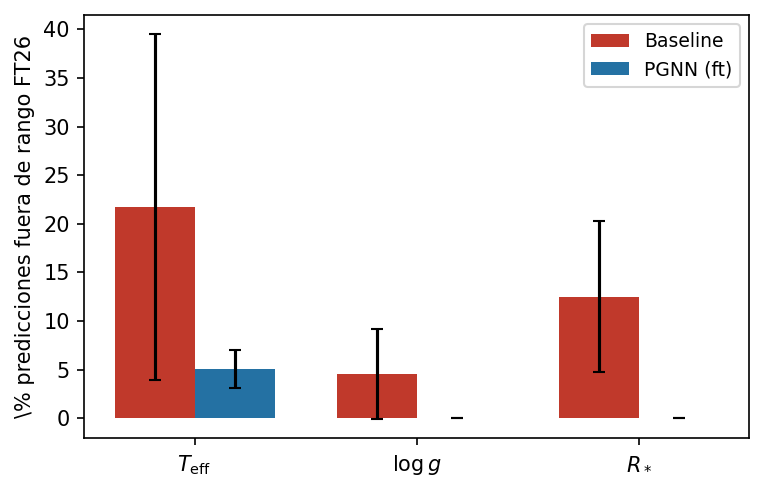
\includegraphics[width=\columnwidth]{fig_oor.png}
  \caption{Tasa de predicciones fuera del rango de validez FT26 sobre IACOB
  (media $\pm$ desv.\ est., 5 semillas). La restricción física elimina las
  violaciones de $\log g$ y $R_*$ y reduce las de $T_\mathrm{eff}$.}
  \label{fig:oor}
\end{figure}

\subsection{Consistencia física y brecha de dominio}

La pérdida física media $\mathcal{L}_\mathrm{phys}$ cae de $2.08$ (Baseline,
prueba sintética) a $\sim\!0.01$ en todas las variantes PGNN, y de forma análoga
sobre UVES~POP ($1.40\to0.02$--$0.06$) e IACOB ($0.59\to0.01$). Subrayamos que
$\mathcal{L}_\mathrm{phys}$ es el mismo término optimizado en entrenamiento, por
lo que mide coherencia interna y \emph{no} constituye una validación independiente
de $\dot{M}$. La \emph{brecha de dominio} $\Delta_k=\mathrm{MAE}_k^\mathrm{IACOB}-
\mathrm{MAE}_k^\mathrm{synth}$ se reduce en todos los parámetros: para
\emph{ft}, $\Delta_{T_\mathrm{eff}}$ pasa de $9683$ a $2089$\,K, $\Delta_{\log g}$
de $0.39$ a $0.18$ y $\Delta_{R_*}$ de $4.12$ a $2.60\,R_\odot$. La hipótesis
$\Delta_k^\mathrm{PGNN}<\Delta_k^\mathrm{Baseline}$ se cumple en los tres
parámetros con etiqueta real.

\subsection{Sensibilidad a $\lambda_\mathrm{phys}$}

La Tabla~\ref{tab:sweep} barre $\lambda_\mathrm{phys}\in\{0.05,\dots,0.50\}$ y
reporta la MAE normalizada media sobre los tres parámetros con etiqueta IACOB
($T_\mathrm{eff}$, $\log g$, $R_*$; espacio $[0,1]$), evitando privilegiar un solo
parámetro. La ganancia OOD es \emph{robusta} al peso: para cualquier $\lambda$ y
estrategia el error se mantiene en $\sim$0.27--0.29, dentro de la dispersión entre
semillas ---el spread por parámetro es $<\!4\%$ en $T_\mathrm{eff}$, $\log g$ y
$R_*$ por separado. No existe un óptimo agudo; recordamos que
$\lambda_\mathrm{phys}=0.25$ se fija \emph{a priori} (§\ref{subsec:training}), no por
este barrido. Esta robustez es deseable: el método no depende de un ajuste fino del
hiperparámetro físico. La Figura~\ref{fig:tradeoff} resume el compromiso
in-distribution vs.\ OOD en la misma métrica.

\begin{table}[htbp]
  \caption{Sensibilidad a $\lambda_\mathrm{phys}$: MAE normalizada media sobre
  $\{T_\mathrm{eff}, \log g, R_*\}$ en IACOB (espacio $[0,1]$, media 3 semillas).
  $\lambda_\mathrm{phys}=0.25^\star$ se fija \emph{a priori} (§\ref{subsec:training}),
  no por ser el mínimo; la columna \emph{rango} (máx$-$mín) muestra que el error OOD
  varía $<\!0.02$ entre todos los pesos: el método es insensible a
  $\lambda_\mathrm{phys}$.}
  \label{tab:sweep}
  \footnotesize
  \setlength{\tabcolsep}{4pt}
  \begin{tabular}{lrrrrrrr}
    \toprule
    Config. & 0.05 & 0.10 & 0.20 & $0.25^\star$ & 0.30 & 0.50 & rango \\
    \midrule
    \emph{ft}          & 0.278 & 0.274 & 0.277 & 0.275 & 0.279 & 0.281 & 0.007 \\
    \emph{scratch}     & 0.284 & 0.286 & 0.287 & 0.289 & 0.287 & 0.290 & 0.006 \\
    \emph{domain}      & 0.277 & 0.276 & 0.280 & 0.280 & 0.279 & 0.280 & 0.004 \\
    \emph{ft}+obs      & 0.286 & 0.286 & 0.281 & 0.282 & 0.279 & 0.277 & 0.009 \\
    \emph{scratch}+obs & 0.287 & 0.283 & 0.285 & 0.283 & 0.283 & 0.284 & 0.004 \\
    \emph{domain}+obs  & 0.288 & 0.282 & 0.278 & 0.280 & 0.279 & 0.276 & 0.012 \\
    \bottomrule
  \end{tabular}
\end{table}

\begin{figure}[t]
  \centering
  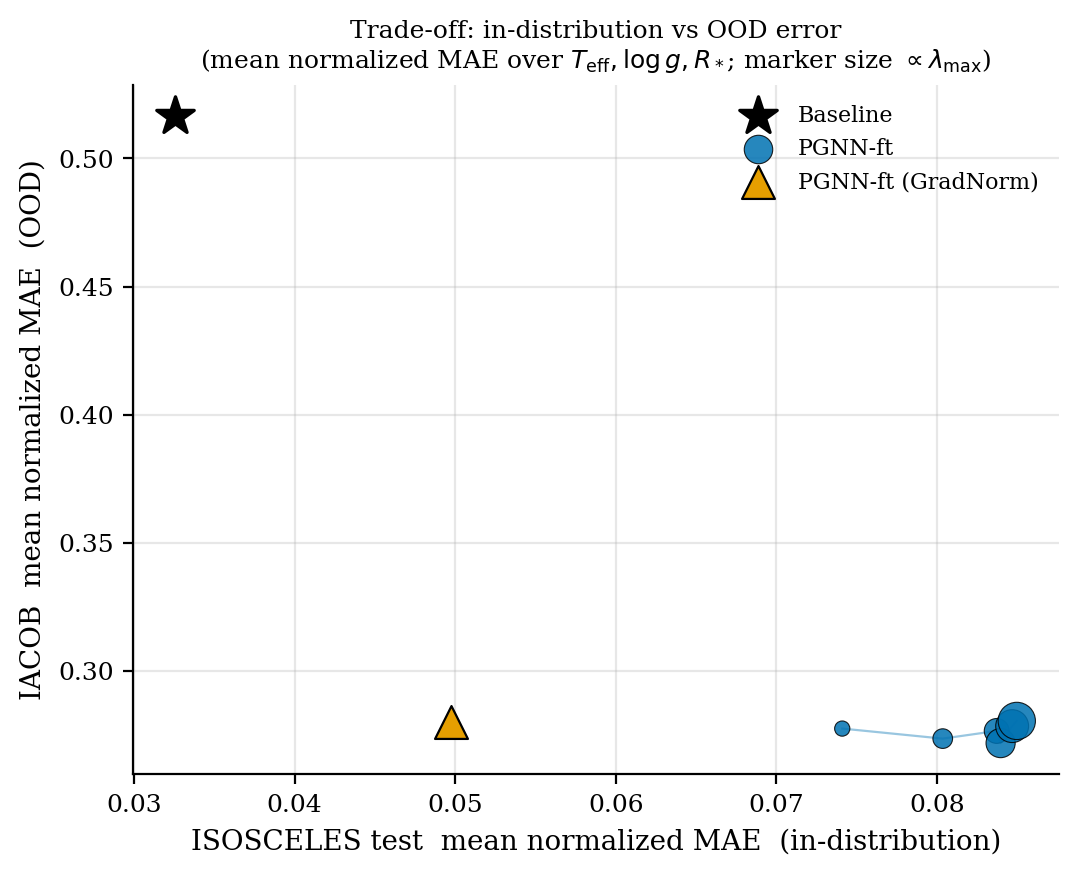
\includegraphics[width=\columnwidth]{fig3_tradeoff.png}
  \caption{Compromiso in-distribution vs.\ OOD para PGNN-\emph{ft}, en MAE
  normalizada media sobre $T_\mathrm{eff}$, $\log g$ y $R_*$ (espacio $[0,1]$).
  El Baseline (estrella) tiene bajo error in-distribution pero OOD catastrófico;
  PGNN reduce el error OOD a la mitad con un costo in-distribution modesto. El
  tamaño del círculo es $\propto\lambda_\mathrm{phys}$: el error OOD permanece
  plano a lo largo del barrido, confirmando la robustez al peso físico
  (Tabla~\ref{tab:sweep}). GradNorm (triángulo, §\ref{subsec:gradnorm}) alcanza
  el mismo error OOD con un costo in-distribution ${\sim}33\%$ menor que el
  mejor $\lambda_\mathrm{phys}$ fijo, dominando al barrido en sentido de
  Pareto.}
  \label{fig:tradeoff}
\end{figure}

\subsection{Balanceo adaptativo de gradientes (GradNorm)}
\label{subsec:gradnorm}

El desbalance residual de ${\sim}83\times$ (Tabla~\ref{tab:grad}) implica que ningún
$\lambda_\mathrm{phys}$ fijo iguala las normas de los gradientes de
$\mathcal{L}_\mathrm{sup}$ y $\mathcal{L}_\mathrm{phys}$. Para resolverlo de forma
directa entrenamos las tres estrategias con GradNorm (§\ref{subsec:loss}), que
reemplaza el escalar fijo por un peso $w_\mathrm{phys}$ ajustado en cada paso para
equilibrar dichas normas. El método converge a $w_\mathrm{phys}\approx 0.01$ en las
tres estrategias ($0.0094$, $0.0109$, $0.0124$ para \emph{ft}, \emph{scratch} y
\emph{domain}), \emph{un orden de magnitud por debajo} de $\lambda_\mathrm{phys}=0.25$,
llevando la razón de gradientes ponderada de ${\sim}83\times$ hacia el equilibrio: ${\sim}1\times$ en el instante de activación (Tabla~\ref{tab:grad}) y ${\sim}0.3\times$ en promedio al converger, donde $\mathcal{L}_\mathrm{phys}$ ya es pequeña y su gradiente disminuye.

La Tabla~\ref{tab:gradnorm} arroja dos conclusiones. Primera, \emph{la corrección
fuera de distribución persiste}: el MAE de $T_\mathrm{eff}$ sobre IACOB permanece en
$\sim$3500--3700\,K (e indistinguible del $\lambda$ fijo dentro de la dispersión
entre semillas; \emph{scratch} incluso mejora, $3732\to3477$), y $\log g$ y $R_*$ se
mantienen. Esto descarta que la ganancia OOD provenga de un valor afortunado de
$\lambda$: es \emph{robusta al mecanismo de balanceo}. Segunda, GradNorm
\emph{reduce a la mitad el costo in-distribution}: al equilibrar las normas en lugar
de imponer una dominancia fija, el MAE de $T_\mathrm{eff}$ sobre la prueba sintética
cae de ${\sim}1470$ a ${\sim}670$\,K ---prácticamente el del Baseline ($660$)--- y el
de $\log g$ de ${\sim}0.078$ a ${\sim}0.040$. En otras palabras, $\lambda_\mathrm{phys}=0.25$
\emph{sobre-pondera} la física: la restricción no necesita dominar el gradiente para
reconfigurar el comportamiento OOD, basta con equilibrarlo. La contrapartida es que
GradNorm no corrige las limitaciones estructurales de $W_1$ (el $W_1$ de
$\log\dot{M}$ permanece alto, ${\sim}0.90$ para \emph{ft}, por la misma
determinación CNO discutida en §\ref{sec:discusion}).

\begin{table}[htbp]
  \caption{$\lambda$ fijo ($=0.25$) frente a GradNorm (peso $w_\mathrm{phys}$
  adaptativo), media sobre $5$ semillas. GradNorm reproduce la corrección OOD
  (MAE IACOB) reduciendo a la mitad el costo in-distribution (MAE ISOSCELES).}
  \label{tab:gradnorm}
  \scriptsize
  \setlength{\tabcolsep}{3pt}
  \begin{tabular}{llrrrrrr}
    \toprule
    & & \multicolumn{2}{c}{in-dist (ISOSCELES)} & \multicolumn{3}{c}{OOD (IACOB)} & \\
    \cmidrule(lr){3-4}\cmidrule(lr){5-7}
    Estrat. & peso & $T_\mathrm{eff}$ & $\log g$ & $T_\mathrm{eff}$ & $\log g$ & $R_*$ & $w_\mathrm{phys}$ \\
    \midrule
    Baseline & --- & 660 & \textbf{0.013} & 10343 & 0.40 & 4.63 & --- \\
    \midrule
    \emph{ft}      & $\lambda{=}0.25$ & 1371 & 0.074 & \textbf{3460} & \textbf{0.25} & \textbf{3.46} & --- \\
    \emph{ft}      & GradNorm & \textbf{657} & 0.038 & 3603 & 0.26 & 3.57 & 0.009 \\
    \emph{scratch} & $\lambda{=}0.25$ & 1526 & 0.080 & 3732 & 0.26 & 3.56 & --- \\
    \emph{scratch} & GradNorm & 696 & 0.043 & 3477 & 0.25 & 3.51 & 0.011 \\
    \emph{domain}  & $\lambda{=}0.25$ & 1511 & 0.079 & 3584 & 0.26 & 3.50 & --- \\
    \emph{domain}  & GradNorm & 660 & 0.041 & 3511 & 0.26 & 3.59 & 0.012 \\
    \bottomrule
  \end{tabular}
\end{table}


\section{Discusión}
\label{sec:discusion}

\subsection{Veredicto sobre la hipótesis}

Los resultados sustentan la hipótesis para los tres parámetros con etiqueta de
literatura ($T_\mathrm{eff}$, $\log g$, $R_*$). La evidencia es convergente y de
cuatro tipos. Primero, el MAE fuera de distribución cae $66\%$, $37\%$ y $25\%$
respectivamente (Tabla~\ref{tab:iacob}). Segundo, y más importante, se
\emph{corrige el sesgo}: el error del Baseline era casi enteramente sistemático
---para $T_\mathrm{eff}$, el sesgo $+10\,091$\,K coincide casi con el MAE de
$10\,343$\,K--- y la restricción física lo reduce a una fracción ($-2318$\,K para
\emph{ft}), recentrando además $\log g$ ($+0.27\to-0.09$) y $R_*$
($-3.77\to-0.07$). Tercero, la admisibilidad física mejora: las violaciones de
rango de $\log g$ y $R_*$ se eliminan por completo y las de $T_\mathrm{eff}$ caen
de $18.6\%$ a $3.8\%$ (Tabla~\ref{tab:oor}). Cuarto, la \emph{brecha de dominio}
$\Delta_k$ ---la cantidad que la hipótesis nombra explícitamente--- se reduce en
los tres parámetros (para \emph{ft}: $\Delta_{T_\mathrm{eff}}$ de $9683$ a
$2089$\,K).

Conviene precisar el sentido de esta confirmación. La evidencia sustenta la
hipótesis en su dimensión \emph{agregada}: admisibilidad física
(Tabla~\ref{tab:oor}), corrección del sesgo sistemático y reducción de la brecha
de dominio $\Delta_k$ (Tabla~\ref{tab:iacob}). No constituye, en cambio, una
afirmación sobre la exactitud por estrella \emph{individual}, que no medimos de
forma directa: el efecto dominante de la restricción es relocalizar las
predicciones dentro del régimen físico admisible y corregir el sesgo poblacional,
no necesariamente ordenarlas estrella a estrella.

El mecanismo es coherente con la literatura de aprendizaje con restricciones
físicas: la prescripción CNO acopla las cuatro cabezas mediante una relación
algebraica válida sólo dentro del régimen O admisible, y minimizar
$\mathcal{L}_\mathrm{phys}$ proyecta las predicciones hacia esa variedad, de modo
análogo a como Masclans et al.~\cite{Masclans2023} y Ballester
et al.~\cite{Ballester2026} restringen sus soluciones, aunque aquí sobre un
problema \emph{inverso} de parámetros superficiales. Es decisivo que esto ocurra
\emph{sin ninguna etiqueta observada}: la restricción es la única señal fuera de
distribución disponible, lo que confirma que la regularización de dominio
basada en física opera en este régimen de cambio severo ---donde la adaptación de
dominio tipo Cycle-StarNet~\cite{OBriain2021} requeriría grandes conjuntos
observados no etiquetados y no garantizaría admisibilidad física. La hipótesis
\emph{no} queda validada, en cambio, para $\dot{M}$, por las razones que se
detallan más adelante (§\ref{sec:discusion}, casos de fallo).

\paragraph{La consistencia física acerca los espectros observados a la variedad sintética.}
La Figura~\ref{fig:tsne} proyecta (t-SNE) el latente de $64$ dimensiones del
encoder para espectros sintéticos y observados. Bajo el Baseline, los espectros
observados quedan \emph{aislados} en una región marginal del espacio latente,
reflejando la brecha sintético--observado en la representación interna. Al
introducir la restricción de consistencia física en la pérdida, el PGNN atrae
los espectros observados hacia la variedad sintética: las nubes de IACOB y
UVES~POP~O se relocalizan adyacentes a los espectros sintéticos, indicando que
el encoder organiza ambos dominios en una geometría latente más coherente.

\begin{figure*}[t]
  \centering
  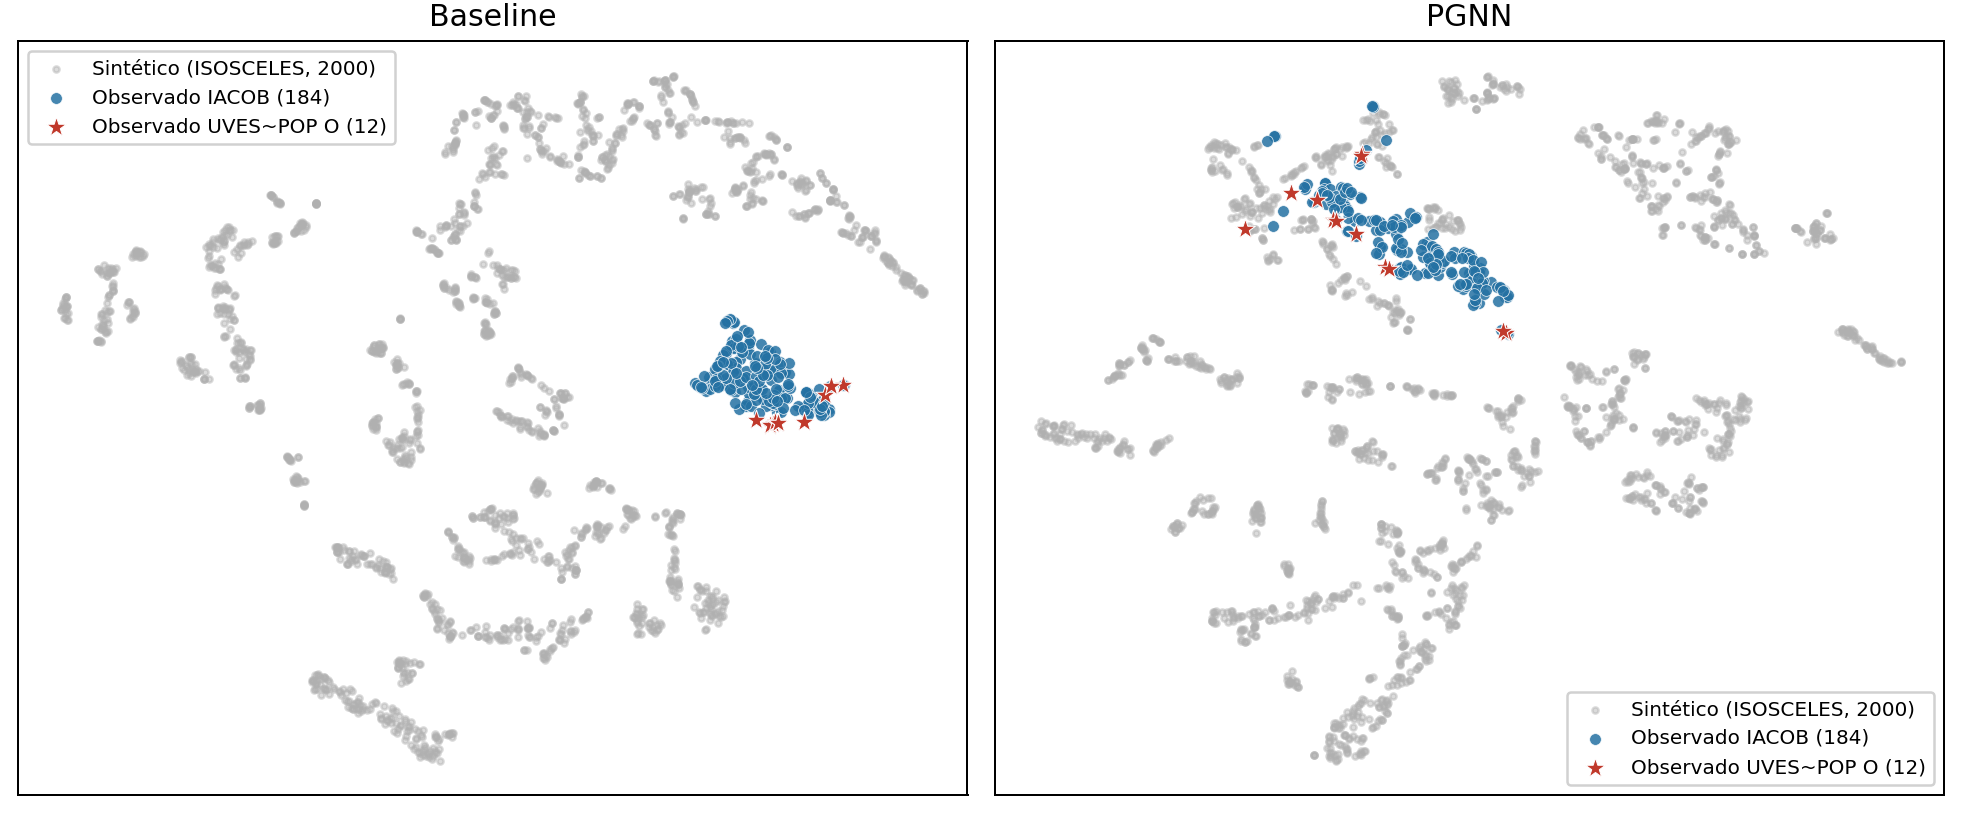
\includegraphics[width=\textwidth]{fig_tsne.png}
  \caption{Embedding t-SNE del latente de $64$ dimensiones del encoder
  (semilla 42): espectros sintéticos (gris) frente a observados (IACOB azul,
  UVES~POP~O rojo), bajo el Baseline y PGNN. El Baseline mantiene los observados
  aislados del soporte sintético; al incorporar la restricción de consistencia
  física, el PGNN los atrae hacia la variedad sintética, reduciendo la brecha
  de dominio en el espacio de representación. Cada panel es un espacio latente
  distinto (sólo la topología es comparable entre paneles).}
  \label{fig:tsne}
\end{figure*}

\subsection{Análisis de componentes}

\paragraph{El término físico domina, no la estrategia de activación.} Tanto el
costo in-distribution (Tabla~\ref{tab:iso}) como la ganancia OOD
(Tabla~\ref{tab:iacob}) son estables a través de \emph{ft}, \emph{scratch} y
\emph{domain}, lo que localiza el efecto en el término físico mismo. El control
con \emph{scratch} (activación diferida, sin \emph{warm-start}) es informativo:
un modelo que nunca visitó un óptimo puramente supervisado converge a la misma
banda OOD que \emph{ft} (que parte del Baseline ya convergido), descartando que la
ganancia sea un artefacto del punto de partida supervisado.

\paragraph{\emph{ft} es la mejor opción y la más barata.} Alcanza el menor
$\mathrm{MAE}(T_\mathrm{eff})$ ($3460$\,K) y reutiliza el Baseline convergido sin
fase de \emph{delay}; lo adoptamos como configuración recomendada. Las
penalizaciones explícitas de \emph{domain} ($R_*\!<\!0$, $\log\dot{M}\!>\!0$) apenas
mueven las métricas OOD sobre \emph{scratch} ---la restricción suave ya mantiene
las predicciones admisibles--- aunque estabilizan $R_*$ (ver fallos).

\paragraph{La física observacional (\emph{+obs}) es un resultado negativo
informativo.} Añadir $\mathcal{L}_\mathrm{phys}$ sobre espectros observados sin
etiqueta deja prácticamente inalteradas todas las métricas OOD ($3460$ para
\emph{ft} vs.\ $3631$ para \emph{ft}+obs; $\log g\!=\!0.26$ en todas las
variantes). La causa es estructural: la prescripción CNO es una relación
algebraica entre las cuatro \emph{salidas}, independiente del espectro de entrada.
Evaluada sobre entradas observadas no aporta ninguna dirección de gradiente que el
término sintético no provea ya ---la superficie de restricción es la misma con
independencia del dominio. Por este canal, los espectros observados no etiquetados
no añaden información. Es un negativo valioso: una restricción física \emph{sobre
las salidas} no puede, por sí sola, explotar datos del dominio objetivo como sí lo
haría la adaptación de dominio en el espacio de \emph{entrada}.

\paragraph{El balanceo de gradientes confirma robustez, no dependencia de
$\lambda$.} La variante GradNorm (§\ref{subsec:gradnorm}) ofrece la prueba más
fuerte de que la corrección OOD no es un artefacto del valor escogido de
$\lambda_\mathrm{phys}$. Al aprender el peso que iguala las normas de los
gradientes, converge a $w_\mathrm{phys}\!\approx\!0.01$ ---$25\times$ menor que
$\lambda_\mathrm{phys}=0.25$--- y aun así reproduce la banda OOD de $T_\mathrm{eff}$
($\sim$3500\,K; \emph{scratch} incluso mejora, $3732\to3477$). El efecto del
término físico es, por tanto, robusto al mecanismo de ponderación. Más aún, al
equilibrar las normas en lugar de imponer una dominancia fija, GradNorm \emph{recupera}
la mitad del costo in-distribution ($\mathrm{MAE}(T_\mathrm{eff})$ sintético
$1371\to657$, prácticamente el del Baseline): la restricción no necesita dominar el
gradiente para reconfigurar el comportamiento OOD, basta con equilibrarlo. Esto
revela que $\lambda_\mathrm{phys}=0.25$ sobre-pondera la física, e identifica el
balanceo adaptativo como la vía natural para extender este trabajo.

\subsection{Casos de fallo}

\paragraph{$W_1$ de $\log\dot{M}$ empeora ($0.67\to0.91$--$1.01$).} Es esperado y
estructural. La prescripción CNO \emph{determina} $\log\dot{M}$ a partir de
$\{T_\mathrm{eff}, \log g, R_*\}$; el modelo no posee supervisión independiente de
$\log\dot{M}$ más allá de ISOSCELES, y FT26 ($R^2=0.929$) discrepa
sistemáticamente de las etiquetas $\log\dot{M}$ de ISOSCELES. Proyectar las
predicciones sobre la superficie CNO desplaza por tanto la distribución de
$\log\dot{M}$ predicha respecto a la de la prueba sintética, aumentando $W_1$. El
mismo mecanismo que corrige $T_\mathrm{eff}$, $\log g$ y $R_*$ relocaliza
$\log\dot{M}$ hacia FT26: es un intercambio controlado, consistente con la
advertencia de §\ref{subsec:formalizacion} sobre el balance entre \emph{dos
prescripciones teóricas}, y no una falla del método.

\paragraph{$W_1$ de $R_*$ es inestable (\emph{scratch} $3.04\to3.39$; \emph{domain}
$\to2.02$).} $R_*$ tiene el acoplamiento CNO más débil (coeficiente $1.44$ frente a
$16.81$ de $T_\mathrm{eff}$) y la menor muestra ($148$ frente a $184$ estrellas),
por lo que su distribución es la menos restringida y la más ruidosa entre semillas.
La penalización explícita de \emph{domain} la estabiliza; \emph{scratch} sin ella
deriva. Esto señala a $R_*$ como el parámetro donde una restricción explícita
adicional rinde mejor.

\paragraph{Costo in-distribution (${\sim}2\times$ en $T_\mathrm{eff}$, ${\sim}6\times$
en $\log g$, ${\sim}3\times$ en $\log\dot{M}$).} Es el impuesto de regularización.
La prueba ISOSCELES comparte la distribución sintética, de modo que toda atracción
hacia una prescripción externa debe costar ajuste in-distribution. El factor
$6\times$ en $\log g$ es grande en términos relativos pero absoluto modesto
($0.013\to{\sim}0.08$), aún muy por debajo del MAE OOD de $\log g$ ($0.25$): la
degradación in-distribution es pequeña frente a la ganancia OOD que compra.

\subsection{Limitaciones}

Cuatro limitaciones acotan el alcance de las conclusiones. Primero,
$\mathcal{L}_\mathrm{phys}$ mide \emph{consistencia interna}, no validación
independiente de $\dot{M}$: es el mismo término optimizado en entrenamiento y no
disponemos de tasas de pérdida de masa observadas (los catálogos IACOB aportan sólo
$T_\mathrm{eff}$, $\log g$, $R_*$). Una validación genuina requeriría $\dot{M}$
medido (anchura equivalente de H$\alpha$, exceso radio/IR), que dejamos como trabajo
futuro. Segundo, las muestras observadas son pequeñas y heterogéneas: UVES~POP~O
aporta sólo $12$ estrellas ---lo que vuelve ruidosas las estimaciones de $W_1$, en
especial $R_*$ sobre $148$ estrellas--- e IACOB combina dos \emph{pipelines}
distintos (Holgado et al.~\cite{Holgado2025} y de~Burgos
et al.~\cite{deBurgos2024}), imponiendo un piso de ruido en las etiquetas. Tercero,
el método \emph{hereda el dominio de FT26}: la restricción es válida sólo para
$T_\mathrm{eff}\in[30,50]$\,kK, $\log g\in[2.9,4.3]$ y $R_*\in[7,70]\,R_\odot$, y no
puede extrapolarse a tipos B/A ni a Wolf-Rayet; la propia métrica de admisibilidad
se define sobre estos límites. Cuarto, el modelo entrega estimaciones puntuales sin
cuantificación de incertidumbre; una cabeza bayesiana ---que Ortiz
et al.~\cite{Ortiz2025} reservan como trabajo futuro--- daría barras de error
calibradas, particularmente relevantes en el régimen de alta varianza de $R_*$ y
$\log\dot{M}$.

\section{Conclusiones}

Investigamos si una restricción física suave, derivada de la prescripción CNO de
Figueroa-Tapia et al.~\cite{FigueroaTapia2026}, reduce la brecha sintética en la
estimación de parámetros de estrellas de tipo O a partir de perfiles H$\alpha$, sin
acceso a etiquetas observadas durante el entrenamiento. La respuesta es afirmativa y
cuantitativamente robusta: el término físico reduce el MAE de $T_\mathrm{eff}$ sobre
IACOB de ${\sim}10\,300$ a ${\sim}3\,500$\,K, revierte un sesgo sistemático de
$+10\,000$ a ${\sim}-2\,300$\,K, y baja la fracción de predicciones fuera del rango
físico de $18.6\%$ a $3.8\%$ en $T_\mathrm{eff}$ y a ${\sim}0\%$ en $\log g$ y $R_*$,
a cambio de un costo in-distribution modesto. El efecto se localiza en el término
físico mismo: es estable entre estrategias de activación (\emph{ft}, \emph{scratch},
\emph{domain}) y ---según el control con GradNorm (§\ref{subsec:gradnorm})--- robusto
al mecanismo de ponderación de gradientes, lo que descarta que dependa de un valor
afortunado de $\lambda_\mathrm{phys}$.

Los resultados negativos delimitan el alcance del método. La física observacional
(\emph{+obs}) no aporta señal adicional, porque la restricción opera sobre las
\emph{salidas} y no sobre la entrada; y la coherencia distribucional de
$\log\dot{M}$ y $R_*$ ---los parámetros con menor acoplamiento CNO y menor muestra---
no mejora de forma consistente. Las extensiones naturales son una validación
independiente de $\dot{M}$ con observables de viento, kernels rotacionales realistas
en la augmentación, una cabeza bayesiana para incertidumbres calibradas, y el
balanceo adaptativo de gradientes como mecanismo de ponderación por defecto.

\section{Declaración de uso de IA}
Este informe fue elaborado con asistencia de Claude (Anthropic, modelos Opus 4.6--4.8). La herramienta se utilizó para: (i) apoyar la redacción y revisión de prosa en distintas secciones, mejorando claridad y estructura; (ii) discutir el posicionamiento del trabajo respecto al estado del arte; y (iii) asistir en la implementación de código experimental ---incluida la variante de balanceo adaptativo GradNorm--- y de los \emph{scripts} de análisis y generación de figuras, bajo dirección de los autores. La pregunta de investigación, la hipótesis, las decisiones de diseño experimental y la interpretación de los resultados fueron desarrolladas por los estudiantes, quienes verificaron todo el contenido técnico y numérico. Las referencias fueron revisadas manualmente y contrastadas con los artículos originales.

\bibliographystyle{ACM-Reference-Format}
\bibliography{sample-base}

\end{document}
\endinput
%%
%% End of file `sample-sigconf-authordraft.tex'.
